\part{Formal Theory of Reconstructive Memory}

\chapter{State Spaces and Transition Systems}\label{ch:transition}

The formal theory begins by fixing what is a state, what is a transition, and what an observer can see. The system state is the tuple $X_t=(M_t,\Psi_t,\Theta_t,Z_t,H_t,B_t)$ of equation~\eqref{eq:state}, taking values in a measurable space $\mathcal X$, and the stochastic variant of the dynamics is the controlled Markov kernel
\begin{equation}\label{eq:kernel}
X_{t+1}\sim P_\vartheta(\,\cdot\mid X_t,c_t,a_t),
\end{equation}
where $c_t\in\Cues\cup\{\varnothing\}$ is the cue presented at step $t$ (or none), $a_t$ is an action drawn from a finite or compact action set that includes encoding an observation, changing the context, and allocating resources, and $\vartheta$ collects the parameters. Three maps complete the specification. The storage map $\Sigma:\mathcal X\times\mathcal O\to\mathcal X$ incorporates an observation $o$ into the persistent component, the observation function $\mathrm{obs}:\mathcal X\to\mathcal W$ reports whatever an external observer is permitted to read directly, and the ecphoric operator $\Eph:\Mem\times\Cues\times\mathcal Z\to\Recs$ produces a reconstruction. The deterministic variant is obtained when $P_\vartheta(\cdot\mid x,c,a)$ is a point mass $\delta_{f_\vartheta(x,c,a)}$, and the finite-dimensional approximation replaces $\mathcal X$ by a finite-dimensional manifold or by a finite set with the cardinalities fixed by the representation sizes of Chapter~\ref{ch:substrate}.

The distinction between the physical state and the accessible mnemonic state is the one that organizes the remaining chapters of the theory. The physical state is $X_t$ in full. The accessible state is its class under recollective equivalence, in the sense of Definition~\ref{def:equiv}: two physical states are mnemonically equivalent if no cue in the admissible family can separate them. For this reading to be coherent the equivalence classes must evolve consistently, so that two equivalent states are still equivalent after the same cue and action. When that holds the accessible state is itself a Markov system, and when it fails the accessible state is not a function of the accessible state at the previous step, so any prediction of recollection from the accessible state alone is incomplete. The condition is exactly the lumpability condition of Chapter~\ref{ch:projection}, and its failure is not a pathology: a memory in which two behaviorally equivalent states respond differently to a future encoding is a memory with hidden state.

\begin{proposition}[Accessible state is a Markov system exactly under lumpability]\label{prop:accmarkov}
Let $\pi:\mathcal X\to\mathcal A$ be the quotient map to accessible states under an equivalence $\sim$ on a finite state space, and let $P$ be a transition kernel for fixed $(c,a)$. The process $\pi(X_t)$ is a Markov chain with transition kernel $\bar P(\alpha,\alpha')=\sum_{x'\in\alpha'}P(x,x')$ for every initial distribution if and only if the sum on the right depends on $x$ only through $\pi(x)$.
\end{proposition}

\begin{proof}
This is the strong lumpability criterion of Kemeny and Snell \cite{kemeny1960}. Sufficiency: if the block-sum is a function of $\pi(x)$, the conditional law of $\pi(X_{t+1})$ given $X_0,\dots,X_t$ depends only on $\pi(X_t)$ and equals $\bar P$. Necessity: if two states $x,y$ in the same block have different block-sums into some block $\alpha'$, an initial distribution concentrated on $x$ and one concentrated on $y$ give the same $\pi(X_0)$ and different laws of $\pi(X_1)$, so $\bar P$ cannot be defined.
\end{proof}

\chapter{Observability and Reconstructive Identifiability}\label{ch:ident}

This chapter contains the central result of the monograph. It is deliberately elementary, in the sense that its proof is a few lines, because its force is in what it makes precise: the difference between a memory that preserves every distinction among histories and a memory that preserves exactly those distinctions that a specified family of future recollections needs.

Let $\Hist$ be a set of histories, $\Mem$ a set of persistent memory states, $\Cues$ a set of admissible cues, and $\Recs$ a set of reconstructions. An encoding is a map $E:\Hist\to\Mem$. A target recollection function $T:\Hist\times\Cues\to\Recs$ specifies what should be reconstructed from the history $h$ when the cue $c$ arrives. An ecphoric decoder is a map $D:E(\Hist)\times\Cues\to\Recs$, and its defining feature, which the theorem makes essential, is that it sees the memory state and the cue and nothing else. In particular it does not see the history.

\begin{definition}[Ecphoric sufficiency]\label{def:suff}
The encoding $E$ is \emph{sufficient} for $T$ on $\Cues$ if $E(h_1)=E(h_2)$ implies $T(h_1,c)=T(h_2,c)$ for all $c\in\Cues$. It is \emph{realized} by a decoder $D$ if $D(E(h),c)=T(h,c)$ for all $h\in\Hist$ and $c\in\Cues$.
\end{definition}

\begin{theorem}[Ecphoric sufficiency criterion]\label{thm:suff}
An encoding $E$ is realized by some decoder if and only if it is sufficient for $T$ on $\Cues$. When it is realized, the decoder is unique on $E(\Hist)\times\Cues$.
\end{theorem}

\begin{proof}
Suppose $D$ realizes $E$ and $E(h_1)=E(h_2)=m$. Then $T(h_1,c)=D(m,c)=T(h_2,c)$ for every $c$, so $E$ is sufficient. Conversely, suppose $E$ is sufficient. For $(m,c)$ with $m\in E(\Hist)$ choose any $h$ with $E(h)=m$ and set $D(m,c)=T(h,c)$. By sufficiency the value does not depend on the choice of $h$, so $D$ is well defined, and $D(E(h),c)=T(h,c)$ by construction. Uniqueness on $E(\Hist)\times\Cues$ holds because any decoder realizing $E$ must take the value $T(h,c)$ at $(E(h),c)$.
\end{proof}

The theorem makes no use of structure on $\Mem$, $\Cues$ or $\Recs$, and this is a feature. The oscillatory, resonant, attractor and inferential mechanisms of Parts~II to V are each a candidate way of computing $D$ within resource limits, and the theorem says that none of them can succeed where the criterion fails. The criterion itself is a purely informational statement about $E$ and $T$. Its content becomes visible in the minimal sufficient memory.

\begin{definition}[Recollective profile and equivalence of histories]\label{def:profile}
The profile of a history is the function $\tau_h=T(h,\cdot):\Cues\to\Recs$. Two histories are recollectively equivalent, $h_1\approx_Th_2$, if $\tau_{h_1}=\tau_{h_2}$.
\end{definition}

\begin{corollary}[Minimal sufficient memory]\label{cor:minimal}
The encoding $E$ is sufficient for $T$ on $\Cues$ if and only if there is a map $\phi:E(\Hist)\to\Hist/\!\approx_T$ with $\phi\circ E=[\cdot]_T$, where $[\cdot]_T$ is the quotient map. Equivalently, $\approx_T$ is a coarsening of the kernel equivalence of $E$. In particular the quotient encoding $[\cdot]_T$ is sufficient and every sufficient encoding factors through it in the sense that it determines it; the cardinality $|\Hist/\!\approx_T|$ is the smallest number of distinct memory states a sufficient encoding can use.
\end{corollary}

\begin{proof}
Sufficiency says that the kernel equivalence of $E$ refines $\approx_T$, which is precisely the existence of $\phi$ with $\phi\circ E=[\cdot]_T$ (a map defined on the image of $E$ by $\phi(E(h))=[h]_T$, well defined by refinement). For the cardinality, $\phi$ is onto $\Hist/\!\approx_T$ because every class contains some $h$, hence $|E(\Hist)|\ge|\Hist/\!\approx_T|$.
\end{proof}


\begin{figure}[t]
\centering
\begin{tikzpicture}[>=Stealth,node distance=3.2cm,every node/.style={font=\small}]
\node (H) {$\Hist$};
\node (M) [right=of H] {$E(\Hist)\subseteq\Mem$};
\node (Q) [below=2.2cm of M] {$\Hist/{\approx_T}$};
\node (Y) [right=3.6cm of M] {$\Recs^{\Cues}$};
\draw[->] (H) -- node[above] {$E$} (M);
\draw[->] (H) -- node[below left] {$[\cdot]_T$} (Q);
\draw[->,dashed] (M) -- node[right] {$\phi$} (Q);
\draw[->] (M) -- node[above] {$D(\cdot,c)_{c\in\Cues}$} (Y);
\draw[->] (Q) -- node[below right] {$\tau$ (injective)} (Y);
\end{tikzpicture}
\caption{Sufficiency as factorization (Theorem~\ref{thm:suff} and Corollary~\ref{cor:minimal}). The profile map $\tau$ sends a class of histories to its recollective profile; $E$ is sufficient exactly when the dashed map $\phi$ exists, and the decoder is then $D=\tau\circ\phi$.}\label{fig:factor}
\end{figure}

The corollary is the formal content of the phrase that memory preserves conditions for reinstatement and not the history itself. Two histories that differ in ways that no admissible cue can reveal through $T$ need not be distinguished by the memory, and any storage that does distinguish them is surplus with respect to $T$. The same distinctions may of course matter for a different target $T'$, which is why the target must be fixed as part of the specification and not left implicit. The example of Chapter~\ref{ch:intro} shows the failure in its smallest form: for $E(a,b)=e_a+e_b$ one has $E(a,b)=E(b,a)$, and a target that returns the first item of the pair has $T((a,b),c)\ne T((b,a),c)$ for every cue that does not reveal order, so no decoder exists however the retrieval dynamics are designed.

The exact criterion is brittle in one respect, since real decoders return approximations. The approximate version is stated for a metric $d$ on $\Recs$.

\begin{theorem}[Approximate sufficiency]\label{thm:approx}
Let $(\Recs,d)$ be a metric space and $\varepsilon\ge0$. For $m\in E(\Hist)$ and $c\in\Cues$ write $A(m,c)=\{T(h,c):E(h)=m\}$. A decoder with $d\bigl(D(E(h),c),T(h,c)\bigr)\le\varepsilon$ for all $h,c$ exists if and only if every set $A(m,c)$ is contained in a closed ball of radius $\varepsilon$. A necessary condition is $\operatorname{diam}A(m,c)\le2\varepsilon$ for all $(m,c)$, and if every set of diameter $\delta$ in $\Recs$ lies in a ball of radius $\delta/2$, which holds on the real line and, more generally, in hyperconvex spaces such as $\ell_\infty^k$, the condition $\operatorname{diam}A(m,c)\le2\varepsilon$ is also sufficient.
\end{theorem}

\begin{proof}
Given such a decoder, the center $D(m,c)$ is within $\varepsilon$ of every element of $A(m,c)$, so the set lies in the ball $\bar B(D(m,c),\varepsilon)$. Conversely, choose for each $(m,c)$ a center $y_{m,c}$ of a closed ball of radius $\varepsilon$ containing $A(m,c)$ and set $D(m,c)=y_{m,c}$. Necessity of the diameter bound follows from the triangle inequality through the center, giving $d(y,y')\le2\varepsilon$ for $y,y'\in A(m,c)$. For the final statement, if $\operatorname{diam}A\le2\varepsilon$ and the set lies in a ball of radius $\operatorname{diam}A/2\le\varepsilon$, the first part applies.
\end{proof}

The factor of two between the necessary and the sufficient conditions is real in general metric spaces and is the price of not assuming that sets of a given diameter have centers close to their elements. In Euclidean space Jung's theorem reduces the gap from a factor of two to a factor of $\sqrt2$, a refinement that does not change the structure of the argument.

The next result quantifies what the absence of sufficiency costs. It concerns the recovery of the history itself, which is the extreme target $T(h,c)=h$.

\begin{proposition}[Identifiability limit]\label{prop:identlimit}
Let $\Hist$ be finite with prior $p$ and let $E$ be deterministic. The maximum over decoders $\hat h:E(\Hist)\to\Hist$ of the probability of recovering $h$ is
\begin{equation}
\max_{\hat h}\Pr[\hat h(E(h))=h]=\sum_{m\in E(\Hist)}\max_{h:E(h)=m}p(h),
\end{equation}
which equals $|E(\Hist)|/|\Hist|$ under the uniform prior. Moreover, for any estimator, Fano's inequality gives
\begin{equation}
\Pr[\hat h(E(h))\ne h]\ \ge\ \frac{H(h\mid E(h))-\log2}{\log|\Hist|}.
\end{equation}
\end{proposition}

\begin{proof}
Given $m$, the decoder must name one history in the fiber $E^{-1}(m)$, and the probability of being correct conditional on $m$ is maximized by the history of greatest prior mass; summing over fibers weighted by the probability of the fiber gives the first expression. Under the uniform prior each fiber has maximum mass $1/|\Hist|$ and there are $|E(\Hist)|$ fibers. Fano's inequality is the standard inequality \cite{cover2006} applied to the variable $h$ and its estimate through $E(h)$, and $H(h\mid E(h))=H(h)-H(E(h))$ for deterministic $E$.
\end{proof}

Two aspects of this bound deserve emphasis. It is independent of the retrieval mechanism, so no amount of recurrent refinement, phase coordination, or learned inference can raise the accuracy above $|E(\Hist)|/|\Hist|$ when only the memory state is consulted. And it concerns recovery of the whole history, so it is an upper bound on the ability to answer every possible question, not on the ability to answer the questions in $T$; Theorem~\ref{thm:suff} is the relevant criterion when the target is narrower. The two together define the extent to which statements about the fidelity of a memory system are statements about the encoding and not about the decoder. A general lesson is that observation of poor reconstruction does not by itself implicate the retrieval dynamics, and a diagnostic that separates the two is to hold the encoding fixed and ask whether Theorem~\ref{thm:suff} is satisfied for the target of interest.

Two qualifications limit how the theorem may be used. The first is that the decoder is assumed to have no additional information; if the decoder can consult the ledger of Chapter~\ref{ch:provenance} or any other store, then that store is part of the memory state and the criterion applies to the combined encoding. The second is that sufficiency is a property of the pair $(E,T)$ together with the cue family, so the claim that a system is sufficient is empty until the cue family is stated, and a system can be sufficient for one family and insufficient for a larger one; this is the formal reason that a design must record the family of future recollections it commits to supporting.

\section*{A finite history space: destroyed and preserved distinctions}\label{sec:finite32}

The criterion is easiest to appreciate on a history space small enough to enumerate. The material of this section is a worked example followed by a proposed extension to noisy encodings; the first is an exercise in Theorem~\ref{thm:suff}, and the second is proved here from elementary decision theory and is not drawn from the memory literature.

\begin{workedex}[Three encodings of a six-element history space]\label{ex:finite32}
Let a history record what was encountered and where, $\Hist=\{a,b,c\}\times\{0,1\}$, so that $h=(x,y)$ has $|\Hist|=6$, and let the prior be uniform. A single future cue asks where the item was seen, so $\Cues=\{c_{\mathrm{where}}\}$ and $T(h,c_{\mathrm{where}})=y$. Consider three encodings: $E_1(x,y)=x$, which keeps the identity of the item and discards the location; $E_2(x,y)=y$, which keeps the location and discards the identity; and $E_3(x,y)=(\bar x,y)$ with $\bar a=\bar b=\mathsf{ab}$ and $\bar c=\mathsf c$, which keeps the location and merges two of the three items. The kernel classes are
\begin{align}
\ker E_1&=\bigl\{\{(a,0),(a,1)\},\{(b,0),(b,1)\},\{(c,0),(c,1)\}\bigr\},\\
\ker E_2&=\bigl\{\{(a,0),(b,0),(c,0)\},\{(a,1),(b,1),(c,1)\}\bigr\},\\
\ker E_3&=\bigl\{\{(a,0),(b,0)\},\{(a,1),(b,1)\},\{(c,0)\},\{(c,1)\}\bigr\},
\end{align}
with $\nnstatesone$, $\nnstatestwo$ and $\nnstatesthree$ classes respectively. The recollective equivalence $\approx_T$ has exactly two classes, $\{y=0\}$ and $\{y=1\}$, since $\tau_h$ depends on $h$ only through $y$. By Corollary~\ref{cor:minimal} an encoding is sufficient exactly when its kernel is contained in $\approx_T$. The kernel of $E_1$ is not contained in $\approx_T$, because the class $\{(a,0),(a,1)\}$ joins two histories with different locations. The kernels of $E_2$ and $E_3$ are contained in $\approx_T$, so both are sufficient, and $E_2$ is the minimal one with $|\Hist/\!\approx_T|=2$ memory states.

For the sufficient encodings the decoder is the one constructed in the proof of Theorem~\ref{thm:suff}: choose a representative of each fiber and read off its location. For $E_2$ it is the table $D_2(0,c_{\mathrm{where}})=0$ and $D_2(1,c_{\mathrm{where}})=1$, and for $E_3$ it is $D_3((\mathsf{ab},y),c_{\mathrm{where}})=D_3((\mathsf c,y),c_{\mathrm{where}})=y$. The tables are explicit and the check $D(E(h),c_{\mathrm{where}})=T(h,c_{\mathrm{where}})$ passes on all six histories. For $E_1$ no table exists. The fiber $\{(a,0),(a,1)\}$ forces a single answer for two different targets, so any decoder errs on at least one of them, and under the uniform prior the best decoder answers correctly with probability one half.
\end{workedex}

The example also separates two quantities that are easily conflated. By Proposition~\ref{prop:identlimit} the accuracy of recovering the whole history is $|E(\Hist)|/|\Hist|$, which equals $\nidaccone$ for $E_1$, $\nidacctwo$ for $E_2$ and $\nidaccthree$ for $E_3$. The encoding that is worst for the stated target, $E_1$, is better than the best minimal encoding at recovering histories, and the ordering of the three encodings by identifiability is not the ordering by sufficiency. This is the quantitative form of the statement that fidelity to the history and sufficiency for a family of recollections are different properties.

\begin{counterex}[Sufficiency is relative to the cue family]\label{cex:cuefamily}
Enlarge the cue family by a second cue, $c_{\mathrm{what}}$, with $T(h,c_{\mathrm{what}})=x$. The recollective equivalence on $\Hist$ is now the identity, since $\tau_h$ determines both coordinates. Then $E_3$, which was sufficient for $c_{\mathrm{where}}$, fails: the class $\{(a,0),(b,0)\}$ joins histories with different answers to $c_{\mathrm{what}}$. The best decoder for the new cue under the uniform prior has error $\nriskthreewhat$, because in each of the two merged classes the decoder must guess between two equally likely items. The encoding $E_2$ fails for the same reason. Only the identity encoding is sufficient for both cues, and it needs all six states. The example shows that the claim ``the encoding is sufficient'' carries an implicit quantifier over the cue family, which is why the family must be recorded in the specification.
\end{counterex}

The three failures above were exact. A deployed memory is noisy, so the memory state is a random variable whose law depends on the history, and the right question is how small the error can be made when the criterion holds only up to a channel.

\begin{extension}[Bayes risk of noisy ecphory]\label{ext:bayesrisk}
Let $\Hist$ be finite with prior $\pi$, and let the encoding be a stochastic kernel $K(m\mid h)$ on a finite set $\Mem$. Fix a cue $c$ and write $y=T(h,c)$. The minimum over all decoders $D:\Mem\to\Recs$ of $\Pr[D(m)\ne T(h,c)]$ is
\begin{equation}
R^\ast(c)\;=\;1-\sum_{m\in\Mem}\max_{y}\ \sum_{h:\,T(h,c)=y}\pi(h)K(m\mid h).
\end{equation}
\emph{(i)} For deterministic $K$ one has $R^\ast(c)=0$ if and only if $E$ is sufficient for $T(\cdot,c)$. For general $K$, $R^\ast(c)=0$ if and only if the conditional laws of $m$ given different target values have disjoint supports. \emph{(ii)} If the target is binary with classes $\Hist_0,\Hist_1$, class priors $\pi_0,\pi_1$ and class-conditional laws $P_j(m)=\Pr[m\mid h\in\Hist_j]$, then $R^\ast=\sum_m\min\{\pi_0P_0(m),\pi_1P_1(m)\}$ and
\begin{equation}\label{eq:bcbound}
\tfrac12\Bigl(1-\sqrt{1-4\pi_0\pi_1\,\mathrm{BC}^2}\Bigr)\ \le\ R^\ast\ \le\ \sqrt{\pi_0\pi_1}\,\mathrm{BC},\qquad \mathrm{BC}=\sum_m\sqrt{P_0(m)P_1(m)}.
\end{equation}
\emph{(iii)} Garbling cannot help: if $K'=GK$ for a further channel $G$ from $\Mem$ to $\Mem'$, then $R^\ast_{K'}(c)\ge R^\ast_K(c)$.
\end{extension}

\begin{proof}
Given $m$, the posterior probability that the target equals $y$ is proportional to
\begin{equation*}
\sum_{h:\,T(h,c)=y}\pi(h)K(m\mid h),
\end{equation*}
so the decoder that names the maximizer is optimal, which gives the first formula. For (i), $R^\ast=0$ forces, for every $m$ with positive mass, that all of the mass at $m$ comes from a single target value, which is the disjoint-support statement; for deterministic $K$ this says each fiber of $E$ lies in one target class, which is Definition~\ref{def:suff}. For (ii), write $a_m=\pi_0P_0(m)$ and $b_m=\pi_1P_1(m)$, so $\sum_m(a_m+b_m)=1$ and $\sum_m\min\{a_m,b_m\}=\tfrac12\bigl(1-\sum_m|a_m-b_m|\bigr)$. Since $|a-b|=\sqrt{(a+b)^2-4ab}$, the Cauchy--Schwarz inequality gives
\begin{equation}
\sum_m|a_m-b_m|\le\Bigl(\sum_m(a_m+b_m)\Bigr)^{1/2}\Bigl(\sum_m\Bigl[(a_m+b_m)-\tfrac{4a_mb_m}{a_m+b_m}\Bigr]\Bigr)^{1/2}=\Bigl(1-4\sum_m\tfrac{a_mb_m}{a_m+b_m}\Bigr)^{1/2}.
\end{equation}
A second application of Cauchy--Schwarz, $\bigl(\sum_m\sqrt{a_mb_m}\bigr)^2\le\sum_m\tfrac{a_mb_m}{a_m+b_m}\sum_m(a_m+b_m)$, gives $\sum_m a_mb_m/(a_m+b_m)\ge\pi_0\pi_1\mathrm{BC}^2$, which yields the lower bound. The upper bound follows from $\min\{a,b\}\le\sqrt{ab}$. For (iii), a decoder for $m'$ composed with $G$ is a randomized decoder for $m$, and randomization cannot beat the optimal deterministic decoder.
\end{proof}

Part (i) is the noisy counterpart of Theorem~\ref{thm:suff}: exact recollection requires that the memory state separate target classes without overlap, and the sufficiency criterion is the case in which the separation is deterministic. Part (iii) is the quantitative content of the remark that retrieval dynamics cannot repair an insufficient encoding: any noise or compression applied downstream of an encoding can only add to its floor. The lower bound in \eqref{eq:bcbound} depends on the encoding only through the Bhattacharyya coefficient of Chapter~\ref{ch:geometry}, which ties practical recoverability to the information geometry of the memory state, and the bound is of the Hellman--Raviv and Kailath type, proved above and checked numerically on two thousand randomly drawn binary channels (Appendix~\ref{app:pilot}).

\begin{workedex}[Noise on a sufficient encoding]\label{ex:noisy32}
Apply the bit-flip channel with flip probability $p=\nbsc$ to the minimal encoding $E_2$ of Worked Example~\ref{ex:finite32}. The two class-conditional laws are $(1-p,p)$ and $(p,1-p)$, the priors are one half, and \eqref{eq:bcbound}-(ii) gives, summing $\min\{\tfrac12(1-p),\tfrac12p\}=\tfrac12p$ over the two memory symbols, $R^\ast=p=\nbsc$. The decoder is the unchanged table $D_2$ read at the noisy symbol. A continuous version places the memory state on the real line, $m=\pm1+\sigma\varepsilon$ with $\varepsilon$ standard normal and $\sigma=\tfrac12$. The optimal decoder is the sign of $m$ and the risk is $\Phi(-1/\sigma)=\ngausstheory$, which a Monte Carlo run of $10^6$ draws reproduces as $\ngaussmc$. Here $\mathrm{BC}=e^{-1/(2\sigma^2)}=\ngaussBC$, and \eqref{eq:bcbound} brackets the risk between $\ngausslb$ and $\ngaussub$. The lower bound is loose by a factor of about five in this regime, which is typical of a bound that holds uniformly over channels, but its direction is the useful one: it shows that the risk cannot be made small without reducing the overlap of the two class-conditional laws.
\end{workedex}

The final quantity connects back to the insufficient encoding. For $E_1$ followed by any symmetric channel the risk remains at least one half, as part (iii) predicts, and the numerical check confirms it for noise levels $0$, $0.1$ and $0.3$. The noisy analysis therefore does not soften the exact theorem; it states how fast failure sets in as the separation between target classes is eroded.

\section*{Dynamic ecphoric sufficiency}

The criterion of Theorem~\ref{thm:suff} concerns a fixed encoding and a fixed family of cues. An adaptive memory changes its state by consolidation, compression, merging and release, and the family of questions it will be asked changes with it. Let $E_0:\Hist\to\Mem_0$ be an initial encoding and let $G_t:\Mem_t\to\Mem_{t+1}$ be transformations of the memory state, chosen from a stream of external observations that does not depend on which history is stored, so that for a given stream the $G_t$ are fixed functions. Write $E_t=G_{t-1}\circ\dots\circ G_0\circ E_0$ for the encoding at time $t$ and $K_t=\ker E_t$ for its kernel equivalence. At each time the system is committed to a target $T_t$ on a cue family $Q_t$, with recollective equivalence $\approx_t$ of Definition~\ref{def:profile}.

\begin{theorem}[Dynamic ecphoric sufficiency]\label{thm:dynsuff}
Let $\approx_{\ge t}=\bigcap_{\tau\ge t}\approx_\tau$ be the equivalence under the joint profile of all future targets, and let the horizon be $T_{\max}\le\infty$. Then
The following hold. (i) the kernels are monotone, $K_t\subseteq K_{t+1}$, so information about the history can only be lost. (ii) $E_\tau$ is sufficient for $(T_\tau,Q_\tau)$ if and only if $K_\tau\subseteq{\approx_\tau}$. (iii) the system can answer every committed family from time $t$ to $T_{\max}$ whatever transformations are applied in between, in the sense that $E_\tau$ is sufficient for $(T_\tau,Q_\tau)$ at every $\tau\ge t$ for every admissible sequence of further transformations, if and only if $K_t\subseteq{\approx_{\ge t}}$ and the further transformations preserve $K_\tau\subseteq{\approx_\tau}$; in particular $K_t\subseteq{\approx_{\ge t}}$ is necessary, and it is sufficient when no further transformation is applied. (iv) a transformation $G_t$ is admissible, meaning that it leaves the system able to answer all committed future families if no further compression is applied, exactly when $\ker(G_t\circ E_t)\subseteq{\approx_{\ge t+1}}$, and the most compressive admissible transformation is the quotient by $\approx_{\ge t+1}$ restricted to the image of $E_t$.
\end{theorem}

\begin{proof}
(i) If $E_t(h_1)=E_t(h_2)$ then $E_{t+1}(h_1)=G_t(E_t(h_1))=G_t(E_t(h_2))=E_{t+1}(h_2)$. (ii) is Theorem~\ref{thm:suff} applied at time $\tau$. (iii) Necessity: by (i) and (ii), sufficiency at every $\tau\ge t$ gives $K_t\subseteq K_\tau\subseteq{\approx_\tau}$ for all $\tau\ge t$, hence $K_t\subseteq\bigcap_{\tau\ge t}{\approx_\tau}$. Sufficiency in the case of no further transformation: then $K_\tau=K_t$ for all $\tau$, and $K_t\subseteq{\approx_{\ge t}}\subseteq{\approx_\tau}$. (iv) Applying (iii) with $E_{t+1}=G_t\circ E_t$ and no further transformation gives the criterion. The quotient of the image of $E_t$ by the relation induced by $\approx_{\ge t+1}$ is well defined exactly when $K_t\subseteq{\approx_{\ge t+1}}$, and any admissible $G_t$ factors through it by Corollary~\ref{cor:minimal}.
\end{proof}

Two consequences deserve statement. The first is irreversibility of insufficiency: if $E_t$ is not sufficient for a target $(T,Q)$, then by (i) no later transformation, however it is chosen, makes the memory sufficient for it, since the kernel only grows. Repair therefore requires information from outside the memory state. The second is the price of an open future.

\begin{corollary}[Cost of commitment]\label{cor:commit}
Let $\mathfrak T\subseteq\mathfrak T'$ be two classes of possible future targets and let $\approx_{\mathfrak T}$ be the equivalence under their joint profile. Then $|\Hist/{\approx_{\mathfrak T}}|\le|\Hist/{\approx_{\mathfrak T'}}|$, so the minimal number of memory states that keeps every target in the class answerable is nondecreasing in the class. If $\mathfrak T'$ contains the identity target $T(h,c)=h$, the minimal memory is the history set itself and no lossless compression exists.
\end{corollary}

\begin{proof}
A larger class gives a finer joint-profile equivalence, since $h\approx_{\mathfrak T'}h'$ implies $h\approx_{\mathfrak T}h'$, so the quotient has at least as many classes. For the identity target the profile separates all histories.
\end{proof}

The corollary is a precise form of the statement that compression is possible only relative to a commitment about what will be asked: a system that wishes to remain answerable to any future question about its past cannot compress, and a system that compresses must have decided, and recorded, which questions it gives up. It is also where the ledger of Chapter~\ref{ch:provenance} enters in a way that no single component supplies.

\begin{proposition}[Repair by the ledger]\label{prop:ledgerrepair}
Suppose the memory state is $(M_t,L_t)$ with $M_t$ a compressed trace store and $L_t$ an append-only ledger whose inscriptions determine the history, so that $\ker E_t^{L}=\mathrm{id}$ for the combined encoding. Then for every target determined by the inscriptions the combined encoding is sufficient at all times, whatever transformations are applied to $M_t$, and a trace store that has lost sufficiency for a newly committed family can be rebuilt from $L_t$. The rebuilt store has the kernel $\approx_{\ge t}$ of the new family, and the cost of repair is the cost of the replay of Proposition~\ref{prop:derived}.
\end{proposition}

\begin{proof}
With the identity kernel, $K_\tau=\mathrm{id}\subseteq{\approx_\tau}$ for every target $\tau$, so (ii) of Theorem~\ref{thm:dynsuff} gives sufficiency, and the ledger is never compressed by the $G_t$ that act on $M_t$ alone. Rebuilding applies an encoding $E'$ defined from the inscriptions, whose kernel is chosen as the quotient by the new joint profile and is therefore sufficient by Corollary~\ref{cor:minimal}.
\end{proof}

The proposition separates two roles that the ledger and the traces play and ties them to the two notions of Chapter~\ref{ch:ident}. Information preservation is guaranteed by the ledger and never lost; resource-bounded accessibility is provided by the traces, which may lose sufficiency irreversibly but can be rebuilt at a cost. What the results do not establish is a rate: how often a trace store must be rebuilt, and what the optimal compression policy is when future families arrive stochastically, are open (Problem~\ref{prob:dynuncertain}). The theorem also assumes that the stream of observations used by the transformations is independent of the stored history; transformations driven by the system's own retrievals, which depend on the history through the memory state, require a different analysis.

\chapter{Stability of Recurrent Reconstruction}\label{ch:stability}

Many of the decoders considered in the monograph are iterated maps. A recurrent reconstruction computes $r^{(k+1)}=F(r^{(k)},c)$ from an initial state, and the questions of this chapter are whether the iteration converges, to what, and with what sensitivity to its inputs. The simplest sufficient condition is contraction. Let $(\mathcal R,d)$ be a complete metric space.

\begin{lemma}[Banach bounds]\label{lem:banach}
If $d(F(x,c),F(y,c))\le\lambda\,d(x,y)$ with $0\le\lambda<1$ for all $x,y$, then $F(\cdot,c)$ has a unique fixed point $r^\star(c)$ and for every initial state $x$ one has $d(F^k(x),r^\star)\le\lambda^kd(x,r^\star)$, the a priori bound $d(F^k(x),r^\star)\le\frac{\lambda^k}{1-\lambda}d(x,F(x))$, and the residual bound $d(x,r^\star)\le\frac{d(x,F(x))}{1-\lambda}$. If in addition $d(F(x,c),F(x,c'))\le L_c\,d(c,c')$ for all $x$, then $d(r^\star(c),r^\star(c'))\le\frac{L_c}{1-\lambda}\,d(c,c')$.
\end{lemma}

\begin{proof}
Existence, uniqueness and the first bound are the Banach fixed-point theorem. For the residual bound, $d(x,r^\star)\le d(x,F(x))+d(F(x),F(r^\star))$, and the last term is at most $\lambda\,d(x,r^\star)$. The a priori bound follows by applying the residual bound at $F^k(x)$ and $d(F^k(x),F^{k+1}(x))\le\lambda^kd(x,F(x))$. For the cue sensitivity, write $\Delta=d(r^\star(c),r^\star(c'))$ and use the triangle inequality through $F(r^\star(c),c')$:
\begin{equation*}
\Delta\le d\bigl(F(r^\star(c),c),F(r^\star(c),c')\bigr)+d\bigl(F(r^\star(c),c'),F(r^\star(c'),c')\bigr)\le L_c\,d(c,c')+\lambda\Delta,
\end{equation*}
and rearrange.
\end{proof}

For the softmax update of Chapter~\ref{ch:attractor} the contraction condition can be made concrete. The map $F(r)=\sum_iw_i(r)m_i$ is smooth with Jacobian $DF(r)=\beta\,\Cov_{w(r)}(m)$, the covariance matrix of the traces under the weights $w(r)$.

\begin{theorem}[Contraction and local stability of the softmax update]\label{thm:contract}
Let $m_1,\dots,m_P$ be unit vectors in $\R^N$.
Part (i): for $\beta<1$ the map $F$ is $\beta$-Lipschitz on $\R^N$, so it has a unique fixed point and the iteration converges to it from every initial state at rate $\beta^k$. Part (ii): at any fixed point $r^\star$ with weights $w^\star=w(r^\star)$, the iteration is locally asymptotically stable if $\beta\,\lambda_{\max}(\Cov_{w^\star}(m))<1$ and locally unstable if $\beta\,\lambda_{\max}(\Cov_{w^\star}(m))>1$.
\end{theorem}

\begin{proof}
The Jacobian is $DF=\beta(\sum_iw_im_im_i^\top-\bar m\bar m^\top)=\beta\Cov_w(m)$ with $\bar m=\sum_iw_im_i$, a positive semidefinite matrix. Its largest eigenvalue is at most its trace, $\operatorname{tr}\Cov_w(m)=\sum_iw_i\norm{m_i}^2-\norm{\bar m}^2\le1$. Hence $\norm{DF}\le\beta$ everywhere, and by the mean value inequality $F$ is $\beta$-Lipschitz, which gives (i) by Lemma~\ref{lem:banach}. For (ii), a fixed point of a $C^1$ map is locally asymptotically stable if the spectral radius of the Jacobian is below one and unstable if some eigenvalue has modulus above one; since $DF=\beta\Cov_{w^\star}$ is symmetric positive semidefinite, its spectral radius is $\beta\lambda_{\max}$.
\end{proof}

Part~(i) says that for $\beta<1$ the memory is a global contraction toward a single blend, since weights hardly depend on the state; this is the regime in which the store behaves as an averaging device. Part~(ii) explains how the blend at low $\beta$ loses stability as $\beta$ grows: at a symmetric blend the covariance $\Cov_{w^\star}(m)$ approaches the covariance of the traces, and the threshold $\beta\lambda_{\max}=1$ is the point at which the blend becomes unstable and single-trace or cluster attractors take over. At a well-separated single-trace attractor the weights concentrate and $\Cov_{w^\star}$ is exponentially small, so the fixed point is strongly stable, which is the one-step cleanup of Proposition~\ref{prop:basin} seen from the dynamical side.

Three propositions are easily run together when a reconstruction is said to converge, and the monograph separates them. A recurrent reconstruction converges dynamically if the iterates approach a fixed point; this is a property of the map $F(\cdot,c)$ alone. It converges representationally if the fixed point lies within a stated distance of a stored trace; this is a property of the map and the store. It converges epistemically if the fixed point lies within a stated distance of the target recollection $T(h,c)$ for the history that produced the memory; this is a property of the map, the store, and the history, and it is the only one of the three that bears on fidelity. The implications run in one direction only: epistemic convergence to a target that is a stored trace entails representational convergence, which entails dynamical convergence of the iteration that reaches it, and none of the converses holds. The contraction regime of Theorem~\ref{thm:contract}(i) in fact sits at the wrong end of this ordering for selective recall, as the following proposition shows.

\begin{proposition}[The globally contractive regime is not selective]\label{prop:blend}
Let $m_1,\dots,m_P$ be unit vectors with maximal pairwise overlap $\mu=\max_{i\ne j}\ip{m_i}{m_j}$, let $\beta<1$, and let $r^\star$ be the unique fixed point of $F$. Then every weight satisfies $w_j(r^\star)\le e^{2\beta}/P<e^2/P$, and for every stored trace
\begin{equation}
\norm{r^\star-m_j}^2\ \ge\ 1-2\mu-2(1-\mu)\,\frac{e^{2}}{P}.
\end{equation}
\end{proposition}

\begin{proof}
The fixed point lies in the convex hull of the traces, so $\norm{r^\star}\le1$ and every score $\ip{m_i}{r^\star}$ lies in $[-1,1]$. Hence $w_j=e^{\beta s_j}/\sum_ie^{\beta s_i}\le e^{\beta}/(Pe^{-\beta})=e^{2\beta}/P$. Then $\ip{m_j}{r^\star}=w_j+\sum_{i\ne j}w_i\ip{m_j}{m_i}\le\mu+(1-\mu)w_j$, and $\norm{r^\star-m_j}^2=\norm{r^\star}^2+1-2\ip{m_j}{r^\star}\ge1-2\mu-2(1-\mu)w_j$.
\end{proof}

For nearly orthogonal traces ($\mu$ small) and a store of more than a few traces the fixed point is therefore at distance close to one from every trace: global convergence is bought by giving up selection. Selective recall requires the multistable regime $\beta\lambda_{\max}>1$ at the blend, in which there are several basins and the guarantees of Proposition~\ref{prop:basin} and Theorem~\ref{thm:capacity} replace the global contraction guarantee.

Contraction is not correctness. The monograph insists on this point because the convergence results above are easy to mistake for evidence of faithful recollection. A contraction converges to its unique fixed point, and the fixed point is a function of the cue and of the stored state, not of the history.

\begin{example}[Contraction without fidelity]\label{ex:constant}
The constant map $F(x,c)=x_0$ is a contraction with $\lambda=0$ for every $c$, converges in one step, and is perfectly stable to cue perturbations, since $L_c=0$. It reconstructs the same state for every history and every cue, and no sufficiency criterion is met for any nonconstant target.
\end{example}

The quantity that connects stability to correctness is the residual at the target. For a target reconstruction $y=T(h,c)$, Lemma~\ref{lem:banach} gives $d(y,r^\star(c))\le d(y,F(y,c))/(1-\lambda)$, so the iteration recovers the target to within $\delta/(1-\lambda)$ when the target is an approximate fixed point of the dynamics with residual $\delta$. In words, contraction amplifies the target's residual by the factor $(1-\lambda)^{-1}$ and no more; design of the update must therefore make the targets approximate fixed points, which is a requirement on how traces are written, not on how the iteration is run. The same lemma bounds the sensitivity to cue perturbation by $L_c/(1-\lambda)$, so that robustness to degraded cues and sharpness of the attractor trade against each other through $\lambda$.

Other regimes need other tools. If the iteration is linear, $F(x)=Ax$, the long-run behavior is governed by the spectrum of $A$: convergence if the spectral radius is below one, sustained oscillation if there is a complex pair on the unit circle, and divergence beyond it. For a gradient system $\dot r=-\nabla V(r)$ the potential $V$ is itself a Lyapunov function with $\dot V=-\norm{\nabla V}^2\le0$, as in the Kuramoto and softmax cases of Chapters~\ref{ch:kuramoto} and~\ref{ch:attractor}, and convergence to the critical set of $V$ follows from standard arguments when $V$ is bounded below with compact sublevel sets. Non-gradient terms, such as the dispersive terms of Chapter~\ref{ch:cgl}, break this guarantee and admit limit cycles and chaotic reconstructions, which are admissible only if the specification assigns them a meaning.

Figure~\ref{fig:contraction} confirms the geometric rate of Theorem~\ref{thm:contract}. The observed convergence is faster than the bound, which holds uniformly over all initial states and all stores.

\begin{figure}[t]
\centering
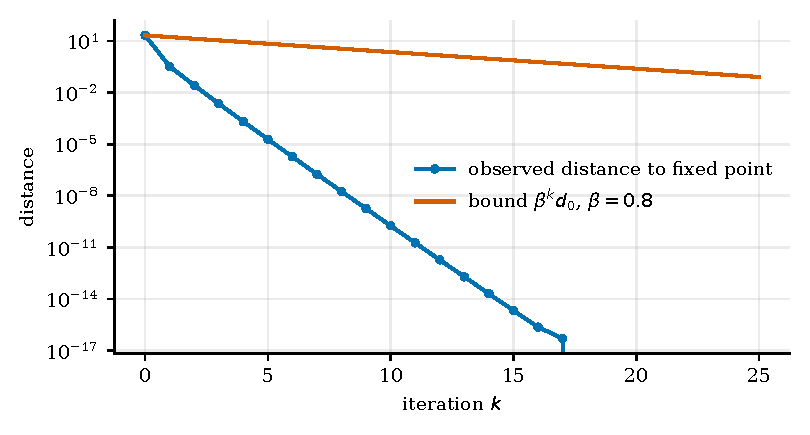
\includegraphics[width=0.85\textwidth]{figs/contraction}
\caption{Distance to the fixed point for the softmax update with $\beta=0.8$ on twelve unit traces in $\R^{64}$, with the bound $\beta^kd_0$ of Theorem~\ref{thm:contract}(i). Computed by the script \texttt{figs.py} with seed 8; an illustration of the stated analytic result and not an evaluation of the architecture.}\label{fig:contraction}
\end{figure}

\section*{Three traces: the Jacobian, the spectrum, and the loss of stability}\label{sec:three33}

The statements of Theorem~\ref{thm:contract} are easiest to appreciate when every quantity can be computed in closed form. The smallest store with a nontrivial competition among traces consists of three orthonormal traces, and this section works it through. Everything below is a worked example of results already proved, together with one extension, the expansion of the unstable branch near the threshold, which is derived here by a direct series computation.

\begin{workedex}[Three orthonormal traces]\label{ex:three33}
Let $m_1,m_2,m_3$ be the standard basis of $\R^3$ and consider the cue-free update $r\mapsto F(r)=\sum_iw_im_i$ with $w=\mathrm{softmax}(\beta r)$, so that $F(r)=w$ and the state lives on the probability simplex. By Chapter~\ref{ch:stability} the Jacobian at a point with weights $w$ is
\begin{equation}
J(w)=\beta\,\mathrm{Cov}_w(m)=\beta\bigl(\mathrm{diag}(w)-ww^{\top}\bigr),
\end{equation}
since $M^{\top}\mathrm{diag}(w)M=\mathrm{diag}(w)$ for orthonormal traces. At the uniform blend $w=(\tfrac13,\tfrac13,\tfrac13)$ the covariance has eigenvalues $\tfrac13,\tfrac13,0$, the zero belonging to the direction $(1,1,1)$ that leaves the simplex, so the Jacobian has leading eigenvalue $\beta/3$ and the blend is locally stable exactly when $\beta<3$, as Theorem~\ref{thm:contract}(ii) requires with $\lambda_{\max}(\mathrm{Cov})=\tfrac13$. Above that temperature the blend is unstable, and the question is where the iteration goes.

The other fixed points have the symmetric form $r=(a,b,b)$ with $a+2b=1$ and $t=a-b$. Substituting into $a=1/(1+2e^{-\beta t})$ gives the scalar equation
\begin{equation}\label{eq:three33}
t=\frac{1-e^{-\beta t}}{1+2e^{-\beta t}},
\end{equation}
whose solution $t=0$ is the uniform blend, $t>0$ is a state dominated by one trace and $t<0$ is a blend of two traces with the third suppressed. A series expansion about $t=0$ gives $\tfrac{1-e^{-\beta t}}{1+2e^{-\beta t}}=\tfrac{\beta t}{3}\bigl(1+\tfrac{\beta t}{6}+O(t^2)\bigr)$, hence \eqref{eq:three33} reads $t(1-\beta/3)=\tfrac{\beta^2}{18}t^2+O(t^3)$ and the nonzero branch near the threshold is
\begin{equation}
t\ \approx\ \frac{6(3-\beta)}{\beta^2},
\end{equation}
which changes sign at $\beta=3$. The bifurcation at $\beta=3$ is therefore transcritical and not a pitchfork, because the branch passes through the blend rather than emerging symmetrically from it. At $\beta=2.9$ the approximation gives $\ntbranchapprox$ and the exact root is $\ntlowCJ$.

Numerical solution of \eqref{eq:three33}, checked against the iteration itself, gives the following picture. For $\beta<\nonset$ the blend is the only fixed point, and for $\beta=2$ the equation has $\ncnttwo$ nonzero roots. At $\beta\approx\nonset$ a saddle-node creates a pair of positive roots. On the window $\nonset<\beta<3$ the blend (leading Jacobian eigenvalue $\nevblendCJ$ at $\beta=2.9$) and a one-trace state ($t=\nthighCJ$, leading eigenvalue $\nevhighCJ$) are both stable, separated by the unstable branch ($t=\ntlowCJ$, leading eigenvalue $\nevlowCJ$), so the system is bistable and the unstable fixed point lies on the boundary between the two basins. At $\beta=3$ the unstable branch meets the blend, which loses its stability there, and for $\beta>3$ the branch continues to $t<0$ as the family of two-trace blends.

At $\beta=6$ there are three kinds of fixed point besides the blend. The one-trace state $r=(\napos,\nbpos,\nbpos)$ has Jacobian eigenvalues $\nevposone$ and $\nevpostwo$ (and $0$ along the normal), so it is a contraction locally and an attractor. The two-trace blend $r=(\naneg,\naneg,\nbneg)$ has eigenvalues $\nevnegone$ and $\nevnegtwo$; the leading one is $\beta$ times the weight $\naneg$ on either of the two surviving traces, with eigenvector $(1,-1,0)$, and it exceeds one, so the blend is a saddle that separates the basins of the two traces it contains. The uniform blend has leading eigenvalue $\nevuniform=\beta/3$ and is repelling. The retrieval picture at high temperature is therefore three attractors, one per trace, separated by saddles at the pair blends and with a repeller at the center.
\end{workedex}

\begin{figure}[t]
\centering
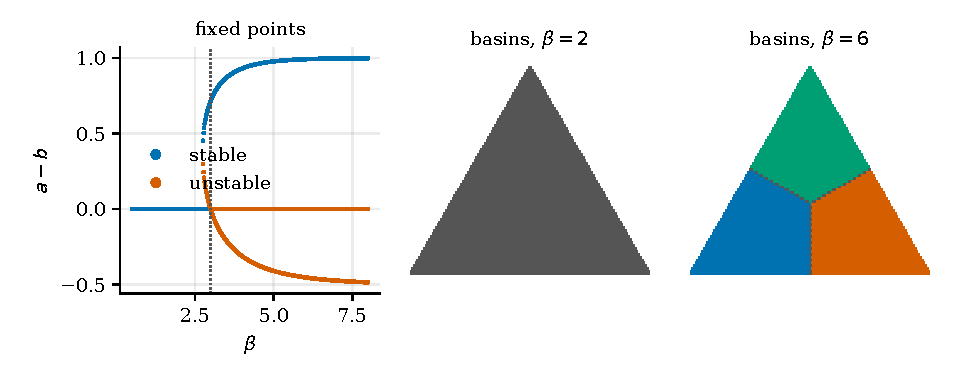
\includegraphics[width=\textwidth]{gen/three_trace}
\caption{The three-orthonormal-trace example. Left: fixed-point branches of \eqref{eq:three33}, expressed as the difference $a-b$, against $\beta$, with stable points in blue and unstable points in orange; the saddle-node near $\beta=\nonset$ and the crossing of the blend at $\beta=3$ are visible. Center and right: basins of attraction of the update on the probability simplex for $\beta=2$ and $\beta=6$. Below the threshold every initial state reaches the uniform blend (grey); above it the simplex divides into three basins. Computed by \texttt{examples.py} with a fixed seed; an illustration of the analytic result.}\label{fig:three33}
\end{figure}

The example shows what the threshold in Theorem~\ref{thm:contract} does and does not control. Crossing $\beta=3$ is the moment at which the blend ceases to be stable, but selection already becomes possible slightly earlier, on the bistable window, where the basin of the one-trace state grows from nothing. The theorem's condition $\beta\lambda_{\max}(\mathrm{Cov}_{w^\star})<1$ is evaluated at a fixed point, and the example shows that different fixed points of the same dynamics have different spectra, so a statement of the form ``the system is stable at temperature $\beta$'' is meaningless without naming the fixed point.

\begin{extension}[Overlap shifts the threshold]\label{ext:overlap33}
Let the three traces have pairwise overlap $\mu\in[0,1)$ and equal norms. By symmetry the blend $r=\bar m$ is still a fixed point with uniform weights, and the covariance of the traces under uniform weights has leading eigenvalue $(1-\mu)/3$. The blend is therefore stable if and only if $\beta<3/(1-\mu)$.
\end{extension}

\begin{proof}
The Gram matrix of the traces is $G=\mu\mathbf 1\mathbf 1^{\top}+(1-\mu)I$. For uniform weights $\mathrm{Cov}(m)=\tfrac13M^{\top}(I-\tfrac13\mathbf 1\mathbf 1^{\top})M$, whose nonzero eigenvalues coincide with those of $\tfrac13(I-\tfrac13\mathbf 1\mathbf 1^{\top})G$. On the subspace orthogonal to $\mathbf 1$ the matrix $G$ acts as $(1-\mu)I$, so the nonzero eigenvalue is $(1-\mu)/3$ with multiplicity two.
\end{proof}

For $\mu=\tfrac12$ the threshold is $\nthrmu$, and the numerical Jacobian at the blend has leading eigenvalue $\nevmuF$ at $\beta=5$ and $\nevmuH$ at $\beta=7$, so it crosses one between them as the formula predicts. The consequence is that correlation among traces postpones the onset of selectivity: the more the stored traces overlap, the colder the system must be, in the sense of a larger $\beta$, before the blend loses stability. This is the dynamical counterpart of the capacity statement of Chapter~\ref{ch:capacity}, that the number of distinguishable traces is controlled by the overlaps.


\chapter{Resonance Selectivity and Capacity}\label{ch:capacity}

The question of capacity is how many traces can be stored before retrieval degrades, and the answer depends on assumptions about the distribution of traces, the noise in the cue, and what counts as success. This chapter derives bounds under explicit assumptions. They are bounds under a random-pattern model and should not be read as measured properties of any particular dataset.

\paragraph{Random-pattern model.} Let the stored traces $m_1,\dots,m_P$ be independent and uniformly distributed on the unit sphere of $\C^n\cong\R^{2n}$. The cap estimate that underlies everything below is that for two independent uniform unit vectors the real overlap satisfies
\begin{equation}\label{eq:cap}
\Pr\bigl[\Re\ip{u}{v}\ge a\bigr]\le(1-a^2)^{n-1}\le e^{-(n-1)a^2},\qquad 0<a<1,
\end{equation}
which follows from the standard bound on the measure of a spherical cap \cite{ball1997}. Equation~\eqref{eq:cap} was verified numerically in the pilot calculations of Appendix~\ref{app:pilot} for $n\in\{16,32,64\}$.

\begin{proposition}[False activation under a resonance threshold]\label{prop:falseact}
Let $\psi,q$ be unit vectors in $\C^n$, so that by Theorem~\ref{thm:closed} the resonance score is $S(\psi,q)=\tfrac12\bigl(1+\Re\ip{\psi}{q}\bigr)$. If a trace is declared active when $S\ge\theta$ with $\theta\in(\tfrac12,1)$, then for a query $q$ independent of $P$ stored random unit traces, the expected number of false activations satisfies
\begin{equation}
\Ex[\#\text{active}]\le P\,e^{-(n-1)(2\theta-1)^2}.
\end{equation}
\end{proposition}

\begin{proof}
$S\ge\theta$ is equivalent to $\Re\ip{\psi}{q}\ge2\theta-1$. Apply \eqref{eq:cap} with $a=2\theta-1$ to each trace and sum over $P$ traces by linearity of expectation.
\end{proof}

The threshold needed to hold the expected number of false activations below one is therefore $2\theta-1\ge\sqrt{\ln P/(n-1)}$, which says that the usable score threshold rises toward one as the store grows at fixed dimension, and the capacity for a given threshold is exponential in the dimension, $P\le e^{(n-1)(2\theta-1)^2}$. This is the exponential capacity in the dimension that is characteristic of dense associative memories \cite{demircigil2017,ramsauer2021}, obtained here for the threshold readout, and its dependence on the squared margin shows the cost of lowering the threshold to tolerate degraded cues.

For the recurrent softmax readout the relevant event is that the stored traces are well separated, so that Proposition~\ref{prop:basin} applies.

The result that follows must be read for what it is. It is a capacity theorem for associative retrieval by a softmax readout over random unit vectors, and the exponential scaling is the familiar consequence of high-dimensional concentration together with a sufficiently low temperature \cite{demircigil2017,ramsauer2021}. It guarantees one-step proximity to a stored trace. It says nothing about recovering temporal organization, historical provenance, or an episode reconstructed from distributed constraints, and it should not be cited as establishing an exponential capacity for episodic recollection. Its role is to show that the retrieval component of the architecture can match known forms of high-dimensional pattern separation, and its price, a temperature that grows linearly with the dimension, is stated in the theorem.

\begin{theorem}[Baseline associative capacity of the softmax readout]\label{thm:capacity}
Let $P=e^{\kappa(n-1)}$ traces be drawn as above, and let $a\in(0,1)$ satisfy $a^2>2\kappa$. Then with probability at least $1-\tfrac12e^{(n-1)(2\kappa-a^2)}$ the maximum overlap satisfies $\max_{i\ne j}\Re\ip{m_i}{m_j}<a$. On this event, for every stored trace $m_j$ and every cue $r$ with $\norm r\le1$ and $\norm{r-m_j}\le\delta$ for some $\delta<(1-a)/2$, one update of the softmax map \eqref{eq:modernhop} with inverse temperature $\beta$ in the realified space satisfies
\begin{equation}
\norm{F(r)-m_j}\le2(P-1)\,e^{-\beta(1-a-2\delta)}.
\end{equation}
In particular the error is below any prescribed $\eta>0$ once $\beta(1-a-2\delta)\ge\kappa(n-1)+\ln(2/\eta)$.
\end{theorem}

\begin{proof}
There are $\binom P2\le P^2/2$ pairs, and the union bound with \eqref{eq:cap} gives the probability that some pair has overlap at least $a$ as at most $\tfrac12P^2e^{-(n-1)a^2}=\tfrac12e^{(n-1)(2\kappa-a^2)}$. On the complement, for the cue $r$ one has $\ip{m_j}{r}=1+\ip{m_j}{r-m_j}\ge1-\delta$ and, for $i\ne j$, $\ip{m_i}{r}=\ip{m_i}{m_j}+\ip{m_i}{r-m_j}\le a+\delta$. The margin is at least $\Delta=1-a-2\delta>0$, and Proposition~\ref{prop:basin} gives the stated bound with $\varepsilon\le(P-1)e^{-\beta\Delta}$. The final statement solves $2Pe^{-\beta\Delta}\le\eta$ for $\beta\Delta$ using $\ln P=\kappa(n-1)$.
\end{proof}

The theorem shows, for associative retrieval of stored traces and not for episodic reconstruction, that the number of recoverable traces can grow exponentially in the dimension, with the rate $\kappa<a^2/2$, provided the inverse temperature grows linearly with the dimension, $\beta\gtrsim\kappa(n-1)/(1-a-2\delta)$. The scaling of $\beta$ is the hidden cost: a memory sharp enough to store exponentially many traces is a memory whose Jacobian $\beta\Cov_w(m)$ is large away from the attractors, so its basins are narrow and its blend states unstable (Theorem~\ref{thm:contract}). Interference accumulates in a different manner under the dilution formula of Proposition~\ref{prop:dilution}: adding a competitor with score $s_n$ rescales the weight of every earlier trace by $Z/(Z+e^{\beta s_n})$, which is small only when the competitor's score is low relative to the incumbents' normalizer. The random-pattern model is the best case for capacity, because it makes overlaps small. Structured stores with clusters of near-duplicates have larger $\mu$ in Proposition~\ref{prop:basin} and require larger margins, and the correlated-pattern and phase-correlated cases are reserved for the experimental program of Chapter~\ref{ch:scaling}.

Figure~\ref{fig:captail} compares the cap bound \eqref{eq:cap} with simulation for three dimensions. The bound holds throughout and has the correct exponential dependence on $n$ and on $a^2$, which is what the capacity argument of Theorem~\ref{thm:capacity} uses.

\begin{figure}[t]
\centering
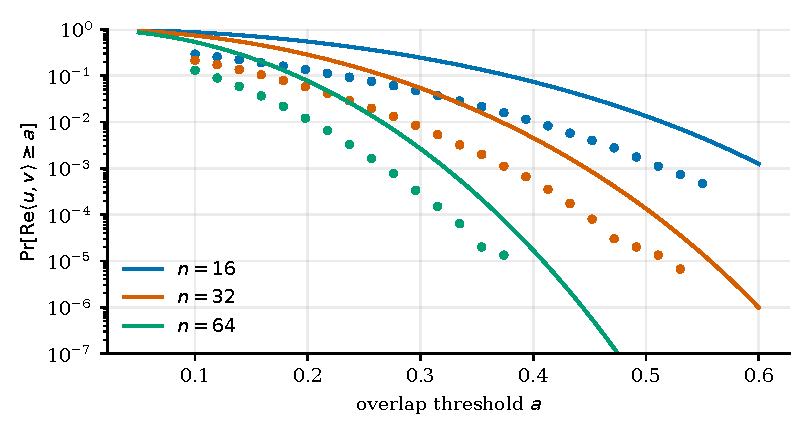
\includegraphics[width=0.85\textwidth]{figs/capacity_tail}
\caption{Empirical tail probability of the real overlap of two independent uniform unit vectors in $\C^n\cong\R^{2n}$ (points, $3\times10^5$ samples) with the cap bound $(1-a^2)^{n-1}$ (curves). Computed by the script \texttt{figs.py} with seed 8; an illustration of the stated analytic result and not an evaluation of the architecture.}\label{fig:captail}
\end{figure}

\section*{Why the margin hypothesis matters}\label{sec:margin34}

The guarantee of Proposition~\ref{prop:basin}, and through it Theorem~\ref{thm:capacity}, is conditional on a margin $\Delta$ between the cued trace and its competitors that exceeds $\beta^{-1}\ln(P-1)$. This section shows by example what happens when the hypothesis fails. It also separates two statements that are easily run together, namely that a sufficient condition has failed and that retrieval has failed. The second statement needs its own proof, and the examples give it by exact computation in a family where everything is available in closed form.

\begin{counterex}[Near-duplicate traces]\label{cex:margin34}
Take $P$ unit traces with a common pairwise overlap $\mu$, that is, with Gram matrix $G=\mu\mathbf 1\mathbf 1^{\top}+(1-\mu)I$, and cue with the first trace, $r=m_1$. The margin is $\Delta=1-\mu$ for every competitor, the weights are $w_1=\bigl(1+(P-1)e^{-\beta(1-\mu)}\bigr)^{-1}$ on the cued trace and $(1-w_1)/(P-1)$ on each other trace, and the one-step error is an exact expression,
\begin{equation}\label{eq:symerr}
\norm{F(m_1)-m_1}=(1-w_1)\sqrt{\frac{1+(P-2)\mu}{P-1}+1-2\mu},
\end{equation}
because $F(m_1)-m_1=(1-w_1)(\bar c-m_1)$ with $\bar c$ the centroid of the competitors. Consider $P=21$ and $\mu=0.9$. The weight on the cued trace equals one half exactly at
\begin{equation}
\beta^\ast=\frac{\ln(P-1)}{1-\mu}=\nbstar,
\end{equation}
and below this temperature the cued trace does not even carry a majority of the weight. At $\beta=20$ one finds $w_1=\nwoneCA$ and a one-step error of $\nerrsymCA$ against a distance $\ndistsym$ from $m_1$ to the centroid of its competitors, so most of the displacement toward the centroid has taken place. The bound of Proposition~\ref{prop:basin} reads $\varepsilon\le(P-1)e^{-\beta\Delta}=\nepsbCA$, which exceeds one and says nothing. At $\beta=40$ the weight is $\nwoneEA$, the error is $\nerrsymEA$ and the bound is $\nepsbEA<1$, so the hypothesis holds and the conclusion is informative. The figure shows the weight $w_1$ against $\beta$ for four store sizes together with the threshold $\ln(P-1)/(1-\mu)$ for each, which grows with the logarithm of the store.
\end{counterex}

\begin{figure}[t]
\centering
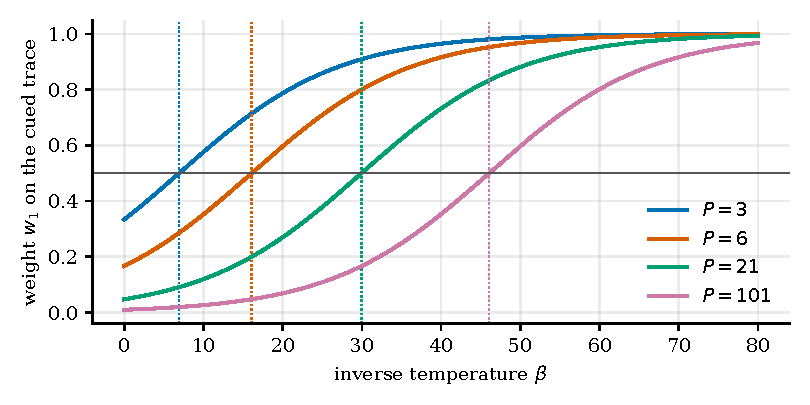
\includegraphics[width=0.85\textwidth]{gen/margin_threshold}
\caption{Weight on the cued trace against inverse temperature for the symmetric near-duplicate family with $\mu=0.9$ and $P\in\{3,6,21,101\}$. The dotted verticals mark $\beta^\ast=\ln(P-1)/(1-\mu)$, where the weight equals one half. Computed by \texttt{examples.py}; an illustration of the closed form in Counterexample~\ref{cex:margin34}.}\label{fig:margin34}
\end{figure}

The counterexample is stated as a necessary scale and not only as a failure. If the hypothesis $\beta\Delta>\ln(P-1)$ is violated by a symmetric family, then $w_1<\tfrac12$, so the single-step update moves the state further than halfway to the competitor centroid; the margin condition is therefore not an artifact of the proof but the temperature at which a symmetric cluster stops being resolved. The same expression also shows why sharpening the temperature is a costly remedy. For this family the cue-free iteration $r\mapsto F(r)$ started at $m_1$ converges for every $\beta$ tested (from $10$ to $40$) to the uniform blend, at distance $\nblendfpdist$ from $m_1$, because the blend remains stable until $\beta$ reaches $1/\lambda_{\max}=P/(1-\mu)=\nblendthr$, where $\lambda_{\max}=(1-\mu)/P$ is the leading covariance eigenvalue at uniform weights, the computation of Extension~\ref{ext:overlap33} with $P$ in place of three. In a store of near-duplicates the temperature at which the cue-free iteration becomes selective is therefore much higher than the temperature at which one step resolves the cue, and whether a cue-anchored iteration of the type in Proposition~\ref{prop:map} holds the cued trace in this regime is not decided by the computation above.

\begin{counterex}[A vacuous bound without a failed retrieval]\label{cex:vacuous34}
A conclusion that the proposition cannot certify is not a conclusion that is false. Take two traces with overlap $\mu=0.9$, so $\norm{m_1-m_2}=\ntwodist$, cue with $r=m_1$ and let $\beta=10$. The margin is $\Delta=0.1$, and the bound of Proposition~\ref{prop:basin} is $\norm{F(r)-m_1}\le2(P-1)e^{-\beta\Delta}=\ntwobound$. This exceeds the distance $\ntwodist$ between the two traces, which is the largest displacement possible for a convex combination of them, so the bound is vacuous. The exact computation gives a weight $\ntwow$ on the competitor and a one-step error $\ntwoerr$, nearly four times smaller than the distance between the traces. The output is closer to $m_1$ than to $m_2$, so the retrieval selects the right trace even though the proposition certifies nothing.
\end{counterex}

The two counterexamples together state what the margin hypothesis can and cannot be used for. Counterexample~\ref{cex:vacuous34} shows that a margin too small to make the bound informative is compatible with correct identification of the nearest trace. Counterexample~\ref{cex:margin34} shows that small margins are not harmless either: in the near-duplicate family the uninformative regime coincides with an exactly computed one-step error comparable to the whole displacement toward the competitor centroid, and with a drift of the cue-free iteration to the blend. The logical situation is that Proposition~\ref{prop:basin} is a sufficient condition, so an uninformative bound licenses no inference by itself, and a conclusion of retrieval failure must be supported by a separate computation, as it is in \eqref{eq:symerr}. For this reason the experimental program of Part~IX reports the margin and the observed error together and does not treat the margin as a predictor.


\chapter{Information Geometry of Memory}\label{ch:geometry}

A memory read out through a softmax or through a Bayesian posterior produces, for each cue, a probability distribution over traces or latent causes. The information geometry of these distributions provides a language for distinguishability that does not depend on the coordinates of the stored embeddings. This chapter develops the elementary parts of that language and states plainly what they do and do not establish.

The softmax weights form an exponential family indexed by the inverse temperature: $p_\beta(i\mid r)=\exp(\beta s_i-\Lambda(\beta))$ with $s_i=\ip{m_i}{r}$ and log-partition $\Lambda(\beta)=\ln\sum_je^{\beta s_j}$. For an exponential family the Fisher information for the natural parameter is the variance of the sufficient statistic, so that
\begin{equation}\label{eq:fishertemp}
\mathcal I(\beta)=\Var_{w}(s)=\Lambda''(\beta),
\end{equation}
which is the amount of information that a single draw of the selected trace carries about the temperature, and which is zero for every $\beta$ if the scores are all equal, tends to zero as $\beta\to\infty$ when the weights collapse onto one trace, and at $\beta=0$ equals the variance of the scores under uniform weights. It can therefore peak at an intermediate temperature where several traces compete, as the example below shows, but it need not do so: the location of the maximum depends on the score profile. This has a consequence for the identifiability analysis of Chapter~\ref{ch:precision}: precision and temperature can be distinguished from outcomes only where this variance is nonzero, and the cue-specific manipulations that make it nonzero are the ones that identify precision.

The space of distributions over a finite set carries a canonical metric, the Fisher--Rao metric $g(\dot p,\dot p)=\sum_i\dot p_i^2/p_i$. The substitution $u_i=2\sqrt{p_i}$ maps the open simplex isometrically onto the positive orthant of the sphere of radius two, since $du_i=dp_i/\sqrt{p_i}$ gives $\sum_idu_i^2=\sum_idp_i^2/p_i$. The geodesic distance is therefore
\begin{equation}\label{eq:fr}
d_{FR}(p,q)=2\arccos\mathrm{BC}(p,q),\qquad\mathrm{BC}(p,q)=\sum_i\sqrt{p_iq_i},
\end{equation}
where $\mathrm{BC}$ is the Bhattacharyya coefficient. The metric is, up to scale, the only Riemannian metric on the simplex that is invariant under sufficient statistics, a theorem of \v{C}encov that is the usual justification for calling it canonical \cite{amari2016}. The geometry reflects the fact that the probability of confusing two distributions from finite samples is controlled by $\mathrm{BC}$, with large $\mathrm{BC}$ meaning near-indistinguishability.

The monotonicity property of this geometry gives a clean bound on what can be recovered from a posterior.

\begin{proposition}[Data-processing for recollective distinguishability]\label{prop:dpi}
Let $K$ be a stochastic kernel from a finite set $\mathcal X$ to a finite set $\mathcal Y$, and let $p,q$ be distributions on $\mathcal X$. Then $\mathrm{BC}(pK,qK)\ge\mathrm{BC}(p,q)$, and consequently $d_{FR}(pK,qK)\le d_{FR}(p,q)$.
\end{proposition}

\begin{proof}
For each $y$, the Cauchy--Schwarz inequality gives
\begin{equation*}
\sqrt{\Bigl(\sum_xp_xK_{xy}\Bigr)\Bigl(\sum_xq_xK_{xy}\Bigr)}\ \ge\ \sum_x\sqrt{p_xq_x}\,K_{xy}.
\end{equation*}
 Summing over $y$ and using $\sum_yK_{xy}=1$ gives the first inequality, and the second follows because $\arccos$ is decreasing.
\end{proof}

If the cues $c$ and $c'$ induce posteriors $p_c$ and $p_{c'}$ over latent causes of Chapter~\ref{ch:inference}, and the reconstruction is a stochastic function of the cause, then the distributions of reconstructions satisfy the proposition's bound: two cues whose posteriors are close in the Fisher--Rao metric cannot produce reconstructions that are further apart in that metric. The geometry of posteriors thus bounds the distinguishability of recollections from above. The proposition does not say that the geometry of posteriors characterizes accessibility, since it is silent about the computational cost of realizing the kernel, and it does not remove the dependence on the stored embeddings, since the posteriors are computed from them. Whether accessibility admits a characterization in terms of the posterior geometry alone, rather than a bound, is left as Problem~\ref{prob:geometry}.

\begin{workedex}[Fisher information of the temperature and a data-processing check]\label{ex:fisher35}
Take three traces with scores $s=(1.0,\,0.2,\,0)$ against a cue. The Fisher information $\mathcal I(\beta)=\mathrm{Var}_w(s)$ equals $\nfishA$ at $\beta=0$, where the weights are uniform, rises to a maximum of $\nfishpeak$ near $\beta=\nfishpeakb$, and falls to $\nfishDA$ (to four decimals) at $\beta=30$, where the first trace carries essentially all the weight. A numerical second difference of the log-partition function reproduces $\mathcal I(\beta)$ to within $10^{-5}$ at $\beta\in\{0.5,3,10\}$, which checks \eqref{eq:fishertemp}. The practical consequence is the one stated above: a cue of this kind identifies the temperature only in an intermediate band, and the design of a cue family for identifying precision is the design of score profiles whose variance is large where the system is meant to operate. A different profile, for instance $(0.9,0.5,0.1)$, has its maximum at $\beta=0$, which is why the location of the peak cannot be asserted in general.

For the distances, let $p=(0.5,0.3,0.2)$ and $q=(0.2,0.3,0.5)$ be the posteriors over three latent causes induced by two cues, and let the reconstruction be a stochastic function of the cause through the kernel with rows $(0.9,0.1)$, $(0.5,0.5)$ and $(0.1,0.9)$. Then $\mathrm{BC}(p,q)=\nBCbefore$ and $d_{FR}(p,q)=\ndFRbefore$, while the output laws satisfy $\mathrm{BC}(pK,qK)=\nBCafter$ and $d_{FR}(pK,qK)=\ndFRafter$. The distance has shrunk, as Proposition~\ref{prop:dpi} requires, and the shrinkage quantifies how much of the distinction between the two cues is lost by the stochastic reconstruction.
\end{workedex}

\begin{problem}[Geometric characterization of accessibility]\label{prob:geometry}
Define a family of cost-bounded decoders and the induced notion of accessible recollective equivalence. Determine whether the equivalence classes of accessible equivalence are the level sets of a function of the Fisher--Rao geometry of the posteriors $\{p_c\}$ alone, or whether the cost of the decoder introduces invariants of the representation that the posterior geometry does not capture.
\end{problem}

\chapter{Projection, Abstraction, and Sufficient Memory States}\label{ch:projection}

An abstraction is a map $\pi:\mathcal X\to\bar{\mathcal X}$ from detailed memory states to compressed representations. For a deterministic dynamics $F:\mathcal X\to\mathcal X$ the abstraction is dynamically adequate if the compressed state evolves autonomously, that is, if there is a map $\bar F$ on the compressed space with
\begin{equation}\label{eq:commute}
\pi\circ F=\bar F\circ\pi.
\end{equation}

\begin{proposition}[Closure criterion]\label{prop:closure}
A map $\bar F$ satisfying \eqref{eq:commute} exists if and only if $\pi(x)=\pi(y)$ implies $\pi(F(x))=\pi(F(y))$, that is, if the kernel equivalence of $\pi$ is preserved by $F$. When it exists it is unique on $\pi(\mathcal X)$.
\end{proposition}

\begin{proof}
If \eqref{eq:commute} holds and $\pi(x)=\pi(y)$ then $\pi(F(x))=\bar F(\pi(x))=\bar F(\pi(y))=\pi(F(y))$. Conversely, if the implication holds define $\bar F(\pi(x))=\pi(F(x))$, which is well defined by hypothesis.
\end{proof}

For stochastic dynamics the same criterion is the strong lumpability of Proposition~\ref{prop:accmarkov}. The criterion is about closure of the projected dynamics, and closure alone says nothing about whether the projection keeps what a recollection needs. The following example separates the two ideas.

\begin{example}[Closure without sufficiency]\label{ex:trivialproj}
Take any $F$ and the projection $\pi(x)=0$ onto a single point. Then $\bar F(0)=0$ satisfies \eqref{eq:commute}, and the compressed dynamics is trivially closed. It also discards every distinction among states, so no nonconstant target can be recovered. Conversely, the identity projection preserves everything and is closed, but achieves no compression. A projection that is useful must be closed and must keep the equivalence class that the future queries require.
\end{example}

\begin{proposition}[Closure and sufficiency together answer future queries]\label{prop:closeandsuff}
Suppose $\pi\circ F=\bar F\circ\pi$ and the reconstruction factors through the projection, $\Eph(x,c)=\bar\Eph(\pi(x),c)$. Then for every initial state $x_0$, every number of steps $k$ and every cue $c$, the reconstruction after $k$ steps equals $\bar\Eph(\bar F^k(\pi(x_0)),c)$, so the compressed system answers every query that the detailed system answers along the trajectory.
\end{proposition}

\begin{proof}
By induction, $\pi(F^k(x_0))=\bar F^k(\pi(x_0))$, since $\pi(F^{k+1}(x_0))=\bar F(\pi(F^k(x_0)))$. Then $\Eph(F^k(x_0),c)=\bar\Eph(\pi(F^k(x_0)),c)$.
\end{proof}

Exact closure is rare and approximate closure is the realistic notion. Suppose the commutation defect is bounded, $\norm{\pi F(x)-\bar F\pi(x)}\le\varepsilon$ for all $x$, and $\bar F$ is $\bar L$-Lipschitz. Let $x_k=F^k(x_0)$ and $\bar x_k=\bar F^k(\pi(x_0))$.

\begin{proposition}[Drift under approximate commutation]\label{prop:drift2}
Under these assumptions $\norm{\pi(x_k)-\bar x_k}\le\varepsilon\sum_{j=0}^{k-1}\bar L^{\,j}$, which is $\varepsilon(1-\bar L^{k})/(1-\bar L)$ for $\bar L\ne1$ and $k\varepsilon$ for $\bar L=1$.
\end{proposition}

\begin{proof}
Let $e_k=\norm{\pi(x_k)-\bar x_k}$, with $e_0=0$. Then $e_{k+1}\le\norm{\pi F(x_k)-\bar F\pi(x_k)}+\norm{\bar F\pi(x_k)-\bar F(\bar x_k)}\le\varepsilon+\bar Le_k$, and the stated sum follows by induction.
\end{proof}

The compressed model is therefore reliable on a horizon of order $1/\varepsilon$ when $\bar L\ge1$, and on all horizons, with error at most $\varepsilon/(1-\bar L)$, when the compressed dynamics is a contraction. The qualitative implication, that contractive compressed dynamics tolerate imperfect closure indefinitely while expansive dynamics do not, bears on the design of consolidation: the slow store of Chapter~\ref{ch:consolidation} should have contractive replay dynamics if it is to remain a faithful abstraction of the fast store.

\paragraph{A linear example: projection onto the span of the traces.}
The projection that discards cue components orthogonal to the traces is an instance of closure that can be checked exactly. Let $V=\operatorname{span}\{m_1,\dots,m_P\}\subset\R^N$ and let $\Pi$ be the orthogonal projector onto $V$. Because each $m_i\in V$, the scores satisfy $\ip{m_i}{r}=\ip{m_i}{\Pi r}$ for every $r$, so the softmax weights depend on $r$ only through $\Pi r$, and the update obeys
\begin{equation}\label{eq:blind}
F(r)=F(\Pi r),\qquad F(r)\in\operatorname{conv}\{m_i\}\subset V,\qquad\text{hence}\qquad \Pi F=F=F\Pi.
\end{equation}
The projection $\pi=\Pi$ is therefore exactly closed with $\bar F=F|_V$, and the update is blind to the component of the cue normal to $V$. If the cue is corrupted by isotropic noise $\xi$ with $\Ex[\xi\xi^\top]=\sigma^2 I_N$, then $\Ex\norm{\Pi\xi}^2=\sigma^2\dim V$, so the fraction of the noise energy that survives the projection is $\dim V/N$, and the remaining fraction $1-\dim V/N$ is removed in one step. When the stored traces span a low-dimensional subspace of a high-dimensional ambient space, most of the noise is discarded.

This is the linear counterpart of the tangent--normal decomposition developed in the author's companion manuscripts on manifold-aligned prediction \cite{flyxion2026npn,flyxion2026hall}. In that framework the semantic manifold $\mathcal M$ has at each point a tangent space and its orthogonal complement, the normal space; admissible explanatory updates lie in the tangent space, and components of an update in the normal space are those that depart from the lawful structure of the data, which the companion work identifies with hallucination. The span $V$ here is the globally flat special case in which the tangent space is the same at every point and the normal space is its complement. Equation~\eqref{eq:blind} says that Mem8's softmax reconstruction has the no-normal-component property in this special case by construction, so that normal-direction content in an output could only enter through additive noise in the dynamics or from a decoder that is not the softmax readout. The curved case requires local tangent spaces and a projection that depends on the base point, and neither the closure property nor the noise-removal fraction extends to it without curvature corrections; those extensions are stated in the companion work and are not derived here. The claims of the companion manuscripts concerning the empirical behavior of recent generative models are cited as claims of those manuscripts and not asserted independently.

Figure~\ref{fig:noise} checks the linear tangent--normal statement of equation \eqref{eq:blind}. The fraction of noise energy surviving the projection matches $\dim V/N$, so a trace span of low dimension discards most of an isotropic perturbation in one step.

\begin{figure}[t]
\centering
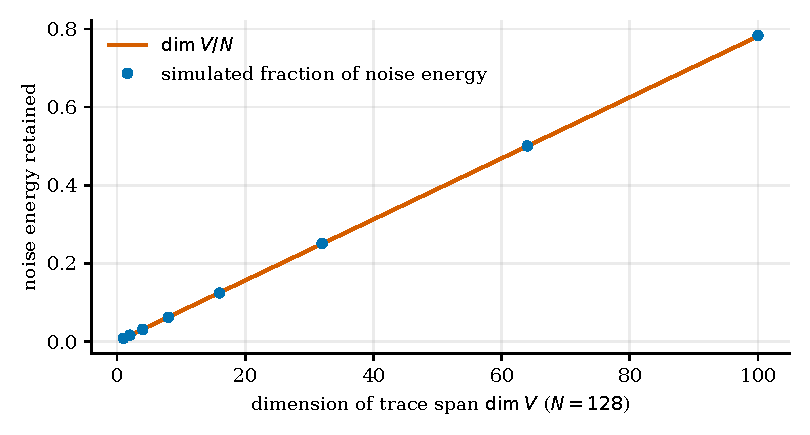
\includegraphics[width=0.85\textwidth]{figs/noise_removal}
\caption{Fraction of isotropic noise energy retained by projection onto the span of the traces in $\R^{128}$, against the dimension of the span, with the value $\dim V/N$ of equation \eqref{eq:blind}. In each run the softmax update was verified numerically to satisfy $F(r)=F(\Pi r)$. Computed by the script \texttt{figs.py} with seed 8; an illustration of the stated analytic result and not an evaluation of the architecture.}\label{fig:noise}
\end{figure}

\section*{Two ways to fail: closure without sufficiency and sufficiency without closure}\label{sec:twofail36}

Example~\ref{ex:trivialproj} separates closure from sufficiency with a degenerate projection that keeps nothing. Two finite constructions make the separation in both directions with projections that are nontrivial, and a stochastic version places it in the language of transition kernels. These are worked examples and a proposed extension; the criteria they exercise are Propositions~\ref{prop:closure} and~\ref{prop:accmarkov} and Theorem~\ref{thm:suff}.

\begin{counterex}[Closed but not sufficient]\label{cex:closedinsuff}
Let $\mathcal X=\{1,2,3,4\}$ with the dynamics $F$ that swaps within the pairs, $F(1)=2$, $F(2)=1$, $F(3)=4$, $F(4)=3$, and let $\pi$ identify each pair, $\pi(1)=\pi(2)=\mathsf A$ and $\pi(3)=\pi(4)=\mathsf B$. Then $\pi(x)=\pi(y)$ implies $\pi(F(x))=\pi(F(y))$, so by Proposition~\ref{prop:closure} the projection is closed, and in fact $\bar F$ is the identity on $\{\mathsf A,\mathsf B\}$. Let the target be the parity of the state within its pair, $T(1)=T(3)=1$ and $T(2)=T(4)=0$. The projection is not sufficient for $T$ by Theorem~\ref{thm:suff}, because the class $\{1,2\}$ contains states with different targets, and the failure is robust: no decoder that sees only the compressed state can answer the parity query at any time, since the compressed trajectory is constant and carries no information about it. The distinction destroyed by $\pi$ is dynamically invisible, which is exactly why closure does not detect its loss. The compressed system is a perfect autonomous model of the block label and an uninformative memory for the parity.
\end{counterex}

\begin{counterex}[Sufficient now but not closed]\label{cex:sufficientnotclosed}
Let $\mathcal X=\{1,2,3,4\}$ with $F(1)=3$, $F(2)=1$, $F(3)=3$, $F(4)=4$, let $T(1)=T(2)=1$ and $T(3)=T(4)=0$, and take the projection $\pi=T$, which has classes $\{1,2\}$ and $\{3,4\}$. The projection is sufficient for $T$ by construction, since the reconstruction is the label itself. It is not closed: $\pi(1)=\pi(2)$ but $\pi(F(1))=\pi(3)=0$ while $\pi(F(2))=\pi(1)=1$. Consequently the compressed system cannot predict its own future label from its present one. The same failure is visible in the language of recollection: the target after one update is $T\circ F$ with $T(F(1))=0$ and $T(F(2))=1$, so $\pi$ is not sufficient for $T\circ F$, and a memory that is sufficient for the recollections required today is not sufficient for the recollections required after one step of its own dynamics.
\end{counterex}

The two counterexamples correspond to two independent defects. Closure is a property of the pair $(\pi,F)$ and says that the kernel of $\pi$ is a congruence for $F$. Sufficiency is a property of the pair $(\pi,T)$ and says that the kernel of $\pi$ refines $\approx_T$. A projection supports recollection along a trajectory only when the kernel of $\pi$ refines $\approx_{T\circ F^k}$ for every $k$ in the horizon, and the coarsest such kernel is the congruence refinement of the targets, which Extension~\ref{ext:viabequiv} of Chapter~\ref{ch:viability} constructs for a system with inputs. The first counterexample shows that closure is not enough and the second that sufficiency at one time is not enough.

For a stochastic dynamics the same two properties are statements about kernels and conditional laws. Let $P$ be a transition kernel on a finite set $\mathcal X$, let $\pi$ partition $\mathcal X$ into blocks, and let $L(x,B')=\sum_{y\in B'}P(x,y)$ be the lumped row. The partition is strongly lumpable if $L(x,\cdot)$ depends on $x$ only through $\pi(x)$, in which case the lumped kernel $\bar P(\pi(x),\cdot)=L(x,\cdot)$ is the transition kernel of $\pi(X_k)$ for every initial law, which is Proposition~\ref{prop:accmarkov}. Sufficiency for a target $T$ at time $k$ is the statement that the conditional law of $T(X_k)$ given $\pi(X_k)$ is degenerate, which is equivalent to the vanishing of the Bayes risk of Extension~\ref{ext:bayesrisk} with the memory state $\pi(X_k)$ and the history $X_k$.

\begin{workedex}[A four-state chain that is lumpable and uninformative]\label{ex:lumped36}
Let $\mathcal X=\{0,1,2,3\}$ with blocks $\{0,1\}$ and $\{2,3\}$, and let the kernel have rows $(0.35,0.35,0.15,0.15)$ for states $0$ and $1$ and $(0.10,0.10,0.40,0.40)$ for states $2$ and $3$. The lumped rows are equal within each block, so the partition is strongly lumpable, with $\bar P=\begin{psmallmatrix}\npbaraa&0.30\\0.20&0.80\end{psmallmatrix}$. The target is the identity of the state within its block, $T(x)=x \bmod 2$. From the uniform initial law the law after one step is $(0.225,0.225,0.275,0.275)$. Given the block label, the two members of each block are equally likely, so the Bayes risk of the parity query is $\nriskblock$, which is the worst possible for a binary target, whereas given the full state it is zero. The compressed chain is therefore an exact autonomous model of the block process and carries no information whatever about the target; the closure of the lumped kernel and the insufficiency of the lumped state hold simultaneously, the stochastic form of Counterexample~\ref{cex:closedinsuff}.
\end{workedex}

Exact lumpability is also fragile, and the realistic notion is the approximate one. For the stochastic case the drift bound of Proposition~\ref{prop:drift2} takes the following form, in which the Lipschitz constant of the compressed dynamics is replaced by the Dobrushin contraction coefficient $\kappa(\bar P)=\max_{a,b}\mathrm{TV}(\bar P(a,\cdot),\bar P(b,\cdot))$.

\begin{extension}[Drift under approximate lumpability]\label{ext:lumpdrift}
Let $P$ be a kernel on a finite set with a partition $\pi$, and let $\bar P$ be a kernel on the blocks with defect $\varepsilon=\max_x\mathrm{TV}\bigl(L(x,\cdot),\bar P(\pi(x),\cdot)\bigr)$. Let $\nu_k$ be the law of $\pi(X_k)$ under $P$ from any initial law of $X_0$, and let $\bar\nu_k=\bar\nu_{k-1}\bar P$ with $\bar\nu_0=\nu_0$. Then
\begin{equation}
\mathrm{TV}(\nu_k,\bar\nu_k)\ \le\ \varepsilon\sum_{j=0}^{k-1}\kappa^j\ =\ \varepsilon\,\frac{1-\kappa^k}{1-\kappa}\ \le\ k\varepsilon,\qquad \kappa=\kappa(\bar P),
\end{equation}
with the middle expression read as $k\varepsilon$ if $\kappa=1$.
\end{extension}

\begin{proof}
Let $\mu_k$ be the law of $X_k$ and $e_k=\mathrm{TV}(\nu_k,\bar\nu_k)$, so $e_0=0$. Then $\nu_{k+1}=\sum_x\mu_k(x)L(x,\cdot)$, and the triangle inequality gives
\begin{equation}
e_{k+1}\le\mathrm{TV}\Bigl(\sum_x\mu_k(x)L(x,\cdot),\ \sum_x\mu_k(x)\bar P(\pi(x),\cdot)\Bigr)+\mathrm{TV}(\nu_k\bar P,\bar\nu_k\bar P)\le\varepsilon+\kappa\,e_k,
\end{equation}
since the middle term is an average of per-state defects and $\sum_x\mu_k(x)\bar P(\pi(x),\cdot)=\nu_k\bar P$, and since $\bar P$ contracts total variation by at most the Dobrushin coefficient. Induction from $e_0=0$ gives the claim.
\end{proof}

\begin{workedex}[Drift in a perturbed chain]\label{ex:drift36}
Perturb state $1$ of Worked Example~\ref{ex:lumped36} to the row $(0.29,0.35,0.21,0.15)$. Its lumped row becomes $(0.64,0.36)$ and the defect against the reference rows of the unperturbed states is $\varepsilon=\ndefect$. The Dobrushin coefficient of the reference kernel is $\kappa=\nkappa$. Starting in the perturbed state, the observed total variation distance between the true block law and the compressed prediction is $\ntvkF$ at $k=5$, against the bound $k\varepsilon=\nbndF$ and the sharper bound $\varepsilon(1-\kappa^k)/(1-\kappa)=\nbndFd$, and it settles at $\ntvinf$ at long horizons. The sharper bound is the informative one: because the compressed kernel contracts, errors do not accumulate linearly, and the asymptotic bound is $\varepsilon/(1-\kappa)=0.12$. The figure shows both bounds against the observed distance.
\end{workedex}

\begin{figure}[t]
\centering
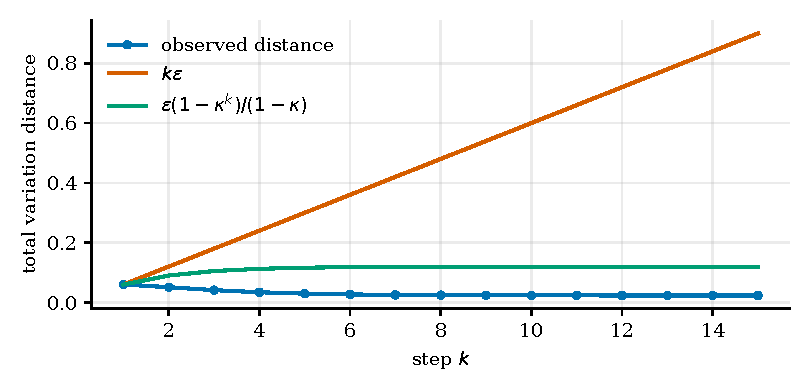
\includegraphics[width=0.85\textwidth]{gen/lump_drift}
\caption{Total variation distance between the true block law and the compressed prediction for the perturbed four-state chain of Worked Example~\ref{ex:drift36}, with the bounds $k\varepsilon$ and $\varepsilon(1-\kappa^k)/(1-\kappa)$ of Extension~\ref{ext:lumpdrift}. Computed by \texttt{examples.py}; an illustration of the stated bound.}\label{fig:lump36}
\end{figure}

The point of the pair of results is the separation of the roles. The bound controls how well the compressed state tracks the block process, which is closure. It does not control what the block process can say about the target, which is sufficiency and has to be certified by the separate criterion of Theorem~\ref{thm:suff}, or by its noisy form in Extension~\ref{ext:bayesrisk}. A system can have an excellent drift bound and a useless memory, as in Worked Example~\ref{ex:lumped36}, or a sufficient memory with an uncontrolled drift, as in Counterexample~\ref{cex:sufficientnotclosed}.


\chapter{Memory as Preservation of Viable Continuation}\label{ch:viability}

A memory is useful when it keeps the system's future options open under its objectives. Stated precisely, a memory policy is a rule that chooses encoding, update and release actions, and its quality is measured by the trajectories it makes possible. Let $f:\mathcal X\times\mathcal A\to\mathcal X$ be a deterministic transition law (stochastic versions replace membership by probability), let $K\subseteq\mathcal X$ be a set of admissible states, and call a trajectory viable if it remains in $K$ for all time.

\begin{definition}[Viability kernel]\label{def:viab}
The viability kernel of $K$ is the set $\Viab(K)$ of initial states from which some sequence of actions yields a trajectory remaining in $K$ forever.
\end{definition}

In the memory setting $K$ encodes constraints such as sufficient remaining resources, bounded interference, and, centrally, a floor on historical fidelity. Define a fidelity functional $D_t\ge0$ measuring the distortion of historically warranted reconstruction, and let $K=\{x:D(x)\le\delta\}\cap K_B$ where $K_B$ collects the resource constraints. The idealized objective of the proposal is
\begin{equation}\label{eq:objective}
\max_{\pi}\ \Ex_\pi\Bigl[\sum_{t=0}^\infty\gamma^t\bigl(U_t-\lambda C_t-\mu D_t\bigr)\Bigr],
\end{equation}
with $U_t$ the continuation value, $C_t$ the computational cost and $D_t$ the distortion. The structure of \eqref{eq:objective} is a penalized formulation in which fidelity trades against utility at the exchange rate $\mu$, and this is exactly what the monograph argues against making the only treatment of fidelity.

\begin{proposition}[Penalties cannot guarantee fidelity]\label{prop:penalty}
Suppose an action $a^\dagger$ yields per-step utility $G$ above the alternative at the cost of per-step distortion $d>\delta$, with all other terms equal. Then the penalized objective \eqref{eq:objective} prefers $a^\dagger$ whenever $\mu<G/d$ (using it at every step), whereas the constrained formulation, which requires the trajectory to stay in $K$, never selects it. For any fixed $\mu$ there exist utility gains $G>\mu d$ at which the penalized optimizer violates the fidelity bound.
\end{proposition}

\begin{proof}
Per step the penalized value of $a^\dagger$ relative to the alternative is $G-\mu d$, which is positive exactly when $\mu<G/d$, and discounting multiplies both sides by $\sum_t\gamma^t$. Under the constrained formulation $a^\dagger$ produces $D=d>\delta$ and leaves $K$, so it is infeasible. Given $\mu$, take $G>\mu d$.
\end{proof}

The proposition is simple, and it shows that with a finite penalty weight the guarantee of fidelity depends on the scale of the utilities, which are not controlled. A hard constraint is a different mathematical object, and its natural solution concept is the viability kernel. For a finite state space the kernel can be computed.

\begin{proposition}[Computation of the viability kernel]\label{prop:viabcomp}
Let $\mathcal X$ be finite and $\mathcal A$ finite. Define $K_0=K$ and $K_{j+1}=\{x\in K_j:\exists a\in\mathcal A,\ f(x,a)\in K_j\}$. The sequence is decreasing, stabilizes after at most $|K|$ steps at a set $K_\infty$, and $K_\infty=\Viab(K)$.
\end{proposition}

\begin{proof}
Each $K_{j+1}\subseteq K_j$, and since the sets are finite the sequence stops decreasing after at most $|K|$ strict decreases; at stabilization every $x\in K_\infty$ has an action leading to $K_\infty$, so repeating the choice yields a viable trajectory and $K_\infty\subseteq\Viab(K)$. Conversely, a state in $\Viab(K)$ has a viable trajectory, and by induction on $j$ every state of that trajectory lies in $K_j$ for all $j$, so $\Viab(K)\subseteq K_\infty$.
\end{proof}

A memory policy that respects the fidelity constraint is one that acts only within $\Viab(K)$, and the operational use of the kernel is to mark actions that appear beneficial in the short run but leave the viable set. For example, a release action that discards a trace is admissible only if the post-release state remains in the kernel, which requires that the discarded distinctions are not needed by any future cue in the committed family, in the sense of Theorem~\ref{thm:suff}. The constrained problem is then to maximize $\Ex\sum_t\gamma^t(U_t-\lambda C_t)$ over policies that stay in $\Viab(K)$, with fidelity a constraint and not a price. Historical fidelity remains separately measurable throughout, which is the property that allows the system to report that a useful reconstruction is historically unwarranted instead of silently trading one for the other.

\section*{Viability-preserving ecphoric equivalence}\label{sec:viabequiv37}

Theorem~\ref{thm:suff} asks which histories a memory must distinguish for the recollections required now, and Proposition~\ref{prop:viabcomp} asks which states the system must be able to leave through an admissible action. The two questions meet in a single one. Two memory states may be indistinguishable to every present recollection and to the present constraint, and yet respond differently once the memory is updated. Whether they may be merged depends on the family of admissible updates, and the answer is a quotient that is in general finer than the sufficiency quotient and coarser than the identity. This section constructs it and states exactly what is new and what is classical.

\paragraph{Setting.} Let $\Sigma=(\mathcal X,\mathcal A,f,K,T)$ be a deterministic system with finitely many memory states $\mathcal X$, a finite set $\mathcal A$ of admissible memory updates (consolidation steps, revisions, searches, releases), a transition law $f:\mathcal X\times\mathcal A\to\mathcal X$, an admissible set $K\subseteq\mathcal X$ and a present recollection map $T:\mathcal X\to\Recs$. Write $o(x)=(T(x),\mathbf 1_K(x))$ for the joint observation of the present recollection and the present admissibility, and $f_w(x)$ for the state reached by the action word $w\in\mathcal A^\ast$.

\begin{definition}[Viability-preserving ecphoric equivalence]\label{def:viabequiv}
Define $x\sim_0y$ if $o(x)=o(y)$ and $x\sim_{n+1}y$ if $x\sim_ny$ and $f(x,a)\sim_nf(y,a)$ for every $a\in\mathcal A$. The relation $\sim_\infty=\bigcap_n\sim_n$ is the viability-preserving ecphoric equivalence.
\end{definition}

\begin{extension}[Viability-preserving ecphoric equivalence]\label{ext:viabequiv}
For finite $\mathcal X$ the following hold. \emph{(i)} The chain $\sim_0\supseteq\sim_1\supseteq\cdots$ stabilizes after at most $|\mathcal X|-1$ refinements, and $\sim_\infty$ is the coarsest equivalence that refines $\sim_0$ and is a congruence for every $f(\cdot,a)$. \emph{(ii)} $x\sim_\infty y$ if and only if $o(f_w(x))=o(f_w(y))$ for every action word $w$; that is, the two states agree on every future recollection and on every future admissibility along every admissible sequence of updates. \emph{(iii)} The viability kernel $\mathrm{Viab}(K)$ of Definition~\ref{def:viab}, its robust counterpart $\{x:f_w(x)\in K\ \forall w\}$, and every set of the form $\{x: T(f_w(x))\in S\}$ are unions of $\sim_\infty$ classes. \emph{(iv)} An encoding $E:\mathcal X\to\Mem$ supports a decoder for $T\circ f_w$ and for $\mathbf 1_K\circ f_w$ for every word $w$ if and only if $\ker E\subseteq\ \sim_\infty$.
\end{extension}

\begin{proof}
(i) The relations $\sim_n$ are equivalences and decrease with $n$. On a finite set a decreasing chain of equivalences that fails to strictly decrease at some step is constant afterwards, because $\sim_{n+1}$ is a function of $\sim_n$ alone, and each strict decrease adds a class, so there are at most $|\mathcal X|-1$ strict decreases. The limit refines $\sim_0$ and is a congruence by construction. If $\equiv$ is another congruence refining $\sim_0$, induction on $n$ shows $\equiv\subseteq\sim_n$ for all $n$, so $\equiv\subseteq\sim_\infty$. (ii) By induction on the length of $w$, $x\sim_ny$ if and only if $o(f_w(x))=o(f_w(y))$ for all words with $|w|\le n$. (iii) If $x\sim_\infty y$ and an action word keeps the trajectory from $x$ inside $K$, then by (ii) the same word keeps the trajectory from $y$ inside $K$, since $\mathbf 1_K$ is part of $o$; the robust kernel and the recollection sets are handled the same way. (iv) If $\ker E\subseteq\ \sim_\infty$ then for each $w$ the targets $T\circ f_w$ and $\mathbf 1_K\circ f_w$ are constant on fibers of $E$ by (ii), so Theorem~\ref{thm:suff} gives decoders. Conversely, if $x\sim_\infty y$ fails there is a word $w$ with $o(f_w(x))\ne o(f_w(y))$, and a decoder for the corresponding target cannot exist on a fiber that contains both.
\end{proof}

\paragraph{Relation to established results.} The ingredients are classical. For a deterministic system with input actions the coarsest congruence refining an observation is the Nerode equivalence of the Moore machine \cite{moore1956}, and the same relation is strong bisimilarity of the labelled transition system with the observation as state label, which is computed by partition refinement \cite{milner1989}. Statement (iii) is the standard fact that bisimilar states have the same viability kernels. What the extension adds is the combination and the reading: the observation $o$ is taken to be the pair of the present recollection and the present admissibility, so that the quotient is at once a sufficiency quotient in the sense of Corollary~\ref{cor:minimal} and a quotient that respects the constraint of Definition~\ref{def:viab}; and the contrast it draws is between the present equivalence $\sim_0$, which is what Theorem~\ref{thm:suff} sees, and the future equivalence $\sim_\infty$, which is what the memory must preserve if it is to be updated. It does not extend to stochastic updates without replacing exact equality of observations by a probabilistic bisimulation, and it does not address learned or approximate updates, for which Problem~\ref{prob:dynuncertain} is the appropriate statement.

\begin{workedex}[Present recollection versus future action]\label{ex:viabequiv37}
Take $\nnstates$ memory states $(b,c)$ with $b\in\{0,1\}$ and $c\in\{1,2,3\}$. The flag $b$ records whether a provisional, uncorroborated trace is held and $c$ counts the steps since it was last attended. The updates are \emph{idle}, which sets $c\leftarrow\min\{c+1,3\}$, and \emph{seek}, which does nothing if $b=0$, resolves the provisional trace to $(0,1)$ if $(b,c)=(1,1)$, and otherwise moves $(1,c)$ to $(1,c-1)$. The admissible set is $K=\{b=0\}\cup\{c\le2\}$, so a provisional trace may not be left unattended to the third count. The present recollection is the flag, $T(b,c)=b$.

The observation $o=(T,\mathbf 1_K)$ separates the states into $\nnTK$ classes at time zero, namely the three states with $b=0$, the pair $\{(1,1),(1,2)\}$ and the state $(1,3)$, whereas $T$ alone separates only $\nnT$. One round of refinement ($\nnrounds$ strict refinement is needed) produces the final partition with $\nncong$ classes,
\begin{equation}
\bigl\{(0,1),(0,2),(0,3)\bigr\},\quad\bigl\{(1,1)\bigr\},\quad\bigl\{(1,2)\bigr\},\quad\bigl\{(1,3)\bigr\}.
\end{equation}
The pair $(1,1)$ and $(1,2)$ is the instructive one. The two states agree on the present recollection and on admissibility, and both belong to the controlled viability kernel, which contains $\nckn$ states, all of $K$. They nevertheless differ under the update \emph{idle}: from $(1,1)$ the result $(1,2)$ is admissible, while from $(1,2)$ the result $(1,3)$ is not, so the first tolerates one unattended step and the second none. A memory that merged them because present recollection could not tell them apart would be sufficient for $T$ and would misjudge, after one update, whether it had left the admissible set. The robust kernel, the states from which every update sequence remains in $K$, is the three states with $b=0$, which form a single class, and both kernels are unions of classes as part (iii) requires. The states with $b=0$ merge entirely, because the counter $c$ is irrelevant to every future observation once the provisional trace has been resolved.
\end{workedex}

\begin{figure}[t]
\centering
\begin{tikzpicture}[>=Stealth,every node/.style={font=\small},st/.style={draw,rounded corners,minimum width=1.6cm,minimum height=0.8cm}]
\node[st,minimum width=4.4cm] (Z) at (3,2.4) {$b=0$ (one class)};
\node[st] (s1) at (0,0) {$(1,1)$};
\node[st] (s2) at (3.2,0) {$(1,2)$};
\node[st,dashed] (s3) at (6.4,0) {$(1,3)$};
\draw[->] (s1) -- node[above] {idle} (s2);
\draw[->] (s2) -- node[above] {idle} (s3);
\draw[->] (s3) to[loop right] node[right] {idle} (s3);
\draw[->,dashed] (s3) to[bend left=35] node[below] {seek} (s2);
\draw[->,dashed] (s2) to[bend left=35] node[below] {seek} (s1);
\draw[->,dashed] (s1) to[bend left=25] node[left] {seek} (Z);
\draw (-0.8,-1.2)--(-0.8,-1.5)--(4.0,-1.5)--(4.0,-1.2);
\node at (1.6,-1.9) {equal under $o=(T,\mathbf 1_K)$, unequal after idle};
\node[font=\footnotesize] at (6.4,-0.75) {outside $K$};
\end{tikzpicture}
\caption{The quotient of Worked Example~\ref{ex:viabequiv37}. The three states with $b=0$ form one class, and the three states with $b=1$ remain distinct. The states $(1,1)$ and $(1,2)$ coincide for the present recollection and the present constraint (bracket) and separate after one \emph{idle} step. The dashed box marks the state outside $K$; self-loops of the class $b=0$ are not drawn.}\label{fig:viabquot}
\end{figure}

The extension also answers a design question that the viability formulation of Chapter~\ref{ch:viability} leaves open. A release action that discards the distinction between two memory states is admissible only if the two states are $\sim_\infty$-equivalent, which is stronger than the requirement that they be equivalent for the committed recollections, and weaker than the requirement that they be identical. In the ledger architecture of Chapter~\ref{ch:provenance} the distinction would be retained as a record of the form that Proposition~\ref{prop:ledgerrepair} allows to be repaired, and the quotient identifies how much of it can be dropped from the working state without loss.


\section*{Synthesis of Part~VII}\label{sec:synth7}

The examples of this part separate four questions that the informal phrase ``the memory works'' runs together, and each has its own certificate. The first is whether the stored state contains what the committed recollections require, which Theorem~\ref{thm:suff} answers exactly and Extension~\ref{ext:bayesrisk} answers with a risk floor when the encoding is noisy. The finite space of Worked Example~\ref{ex:finite32} shows that an encoding can be better at recovering histories and worse at the recollection that matters, and part (iii) of the extension shows that any downstream channel can only raise the floor, so the dynamics of Chapters~\ref{ch:stability} and~\ref{ch:capacity} act on a quantity that is already bounded by the encoding. The second question is whether the retrieval dynamics reach the stored state from the cue, which is a statement about the spectrum of the Jacobian at a fixed point (Worked Example~\ref{ex:three33}) and about margins (Counterexample~\ref{cex:margin34}); both are conditions on the stored traces and the temperature and neither says anything about whether the traces suffice. The third question is whether a compressed state can be evolved without reference to the detailed state, which is closure, certified by lumpability and degraded gracefully by Extension~\ref{ext:lumpdrift}; the two constructions of Chapter~\ref{ch:projection} show that closure and sufficiency are logically independent. The fourth is whether two states that agree on present recollection remain interchangeable under the updates the system may apply, which is the congruence of Extension~\ref{ext:viabequiv} and which strengthens sufficiency by the quantifier over action words.

\begin{table}[t]
\centering
\small
\renewcommand{\arraystretch}{1.25}
\begin{tabularx}{\textwidth}{@{}p{3.1cm}p{3.6cm}X@{}}
\toprule
Question & Certificate & Failure exhibited by the example \\
\midrule
Does the state contain the recollection? & Theorem~\ref{thm:suff}; Extension~\ref{ext:bayesrisk} & Encoding $E_1$ of Example~\ref{ex:finite32} has risk $\nidaccone$ for the location query although it recovers more histories than $E_2$ \\
Does retrieval reach it? & Theorem~\ref{thm:contract}; Proposition~\ref{prop:basin} & Blend unstable above $\beta=3$ for three orthonormal traces; vacuous bound with correct retrieval; drift to the blend for near-duplicates \\
Can the compressed state evolve alone? & Proposition~\ref{prop:closure}; Extension~\ref{ext:lumpdrift} & Closed projection with Bayes risk $\nriskblock$; sufficient projection that is not closed \\
Does equivalence survive updates? & Extension~\ref{ext:viabequiv} & Present-equivalent states $(1,1)$ and $(1,2)$ differ after one idle step \\
\bottomrule
\end{tabularx}
\caption{The four questions of Part~VII, the result that certifies each, and the example that shows the certificate failing independently of the others.}\label{tab:synth7}
\end{table}

Three consequences follow for the design of the system in Part~VIII. First, a diagnostic of poor recollection should be run in order: the encoding is tested against the criterion with the dynamics held fixed, then the dynamics against the margin and spectral conditions with the encoding held fixed, and only then is an architectural change warranted. Second, compression of the working state, whether by lumping, projection or release, should be licensed by the quotient of Extension~\ref{ext:viabequiv} and not by present recollection alone. Third, every quantitative statement in this part is conditional on the model in which it was derived: the three-trace and near-duplicate families are chosen because their spectra are available in closed form, and the extensions are proposed results proved here and not findings about a measured system. Where a statement was checked numerically, the checking script is listed in Appendix~\ref{app:pilot}.

